
%% bare_adv.tex
%% V1.4
%% 2012/12/27
%% by Michael Shell
%% See: 
%% http://www.michaelshell.org/
%% for current contact information.
%%
%% This is a skeleton file demonstrating the advanced use of IEEEtran.cls
%% (requires IEEEtran.cls version 1.8 or later) with an IEEE Computer
%% Society journal paper.
%%
%% Support sites:
%% http://www.michaelshell.org/tex/ieeetran/
%% http://www.ctan.org/tex-archive/macros/latex/contrib/IEEEtran/
%% and
%% http://www.ieee.org/

%%*************************************************************************
%% Legal Notice:
%% This code is offered as-is without any warranty either expressed or
%% implied; without even the implied warranty of MERCHANTABILITY or
%% FITNESS FOR A PARTICULAR PURPOSE! 
%% User assumes all risk.
%% In no event shall IEEE or any contributor to this code be liable for
%% any damages or losses, including, but not limited to, incidental,
%% consequential, or any other damages, resulting from the use or misuse
%% of any information contained here.
%%
%% All comments are the opinions of their respective authors and are not
%% necessarily endorsed by the IEEE.
%%
%% This work is distributed under the LaTeX Project Public License (LPPL)
%% ( http://www.latex-project.org/ ) version 1.3, and may be freely used,
%% distributed and modified. A copy of the LPPL, version 1.3, is included
%% in the base LaTeX documentation of all distributions of LaTeX released
%% 2003/12/01 or later.
%% Retain all contribution notices and credits.
%% ** Modified files should be clearly indicated as such, including  **
%% ** renaming them and changing author support contact information. **
%%
%% File list of work: IEEEtran.cls, IEEEtran_HOWTO.pdf, bare_adv.tex,
%%                    bare_conf.tex, bare_jrnl.tex, bare_jrnl_compsoc.tex,
%%                    bare_jrnl_transmag.tex
%%*************************************************************************

% *** Authors should verify (and, if needed, correct) their LaTeX system  ***
% *** with the testflow diagnostic prior to trusting their LaTeX platform ***
% *** with production work. IEEE's font choices can trigger bugs that do  ***
% *** not appear when using other class files.                            ***
% The testflow support page is at:
% http://www.michaelshell.org/tex/testflow/



% IEEEtran V1.7 and later provides for these CLASSINPUT macros to allow the
% user to reprogram some IEEEtran.cls defaults if needed. These settings
% override the internal defaults of IEEEtran.cls regardless of which class
% options are used. Do not use these unless you have good reason to do so as
% they can result in nonIEEE compliant documents. User beware. ;)
%
%\newcommand{\CLASSINPUTbaselinestretch}{1.0} % baselinestretch
%\newcommand{\CLASSINPUTinnersidemargin}{1in} % inner side margin
%\newcommand{\CLASSINPUToutersidemargin}{1in} % outer side margin
%\newcommand{\CLASSINPUTtoptextmargin}{1in}   % top text margin
%\newcommand{\CLASSINPUTbottomtextmargin}{1in}% bottom text margin



% Note that the a4paper option is mainly intended so that authors in
% countries using A4 can easily print to A4 and see how their papers will
% look in print - the typesetting of the document will not typically be
% affected with changes in paper size (but the bottom and side margins will).
% Use the testflow package mentioned above to verify correct handling of
% both paper sizes by the user's LaTeX system.
%
% Also note that the "draftcls" or "draftclsnofoot", not "draft", option
% should be used if it is desired that the figures are to be displayed in
% draft mode.
%
\documentclass[12pt,journal,compsoc]{IEEEtran}
% The Computer Society requires 12pt.
% If IEEEtran.cls has not been installed into the LaTeX system files,
% manually specify the path to it like:
% \documentclass[10pt,journal,compsoc]{../sty/IEEEtran}


% For Computer Society journals, IEEEtran defaults to the use of 
% Palatino/Palladio as is done in IEEE Computer Society journals.
% To go back to Times Roman, you can use this code:
%\renewcommand{\rmdefault}{ptm}\selectfont





% Some very useful LaTeX packages include:
% (uncomment the ones you want to load)



% *** MISC UTILITY PACKAGES ***
%
%\usepackage{ifpdf}
% Heiko Oberdiek's ifpdf.sty is very useful if you need conditional
% compilation based on whether the output is pdf or dvi.
% usage:
% \ifpdf
%   % pdf code
% \else
%   % dvi code
% \fi
% The latest version of ifpdf.sty can be obtained from:
% http://www.ctan.org/tex-archive/macros/latex/contrib/oberdiek/
% Also, note that IEEEtran.cls V1.7 and later provides a builtin
% \ifCLASSINFOpdf conditional that works the same way.
% When switching from latex to pdflatex and vice-versa, the compiler may
% have to be run twice to clear warning/error messages.






% *** CITATION PACKAGES ***
%
\ifCLASSOPTIONcompsoc
  % IEEE Computer Society needs nocompress option
  % requires cite.sty v4.0 or later (November 2003)
  \usepackage[nocompress]{cite}
\else
  % normal IEEE
  \usepackage{cite}
\fi
% cite.sty was written by Donald Arseneau
% V1.6 and later of IEEEtran pre-defines the format of the cite.sty package
% \cite{} output to follow that of IEEE. Loading the cite package will
% result in citation numbers being automatically sorted and properly
% "compressed/ranged". e.g., [1], [9], [2], [7], [5], [6] without using
% cite.sty will become [1], [2], [5]--[7], [9] using cite.sty. cite.sty's
% \cite will automatically add leading space, if needed. Use cite.sty's
% noadjust option (cite.sty V3.8 and later) if you want to turn this off
% such as if a citation ever needs to be enclosed in parenthesis.
% cite.sty is already installed on most LaTeX systems. Be sure and use
% version 4.0 (2003-05-27) and later if using hyperref.sty. cite.sty does
% not currently provide for hyperlinked citations.
% The latest version can be obtained at:
% http://www.ctan.org/tex-archive/macros/latex/contrib/cite/
% The documentation is contained in the cite.sty file itself.
%
% Note that some packages require special options to format as the Computer
% Society requires. In particular, Computer Society  papers do not use
% compressed citation ranges as is done in typical IEEE papers
% (e.g., [1]-[4]). Instead, they list every citation separately in order
% (e.g., [1], [2], [3], [4]). To get the latter we need to load the cite
% package with the nocompress option which is supported by cite.sty v4.0
% and later.
%
% Note also the use of a CLASSOPTION conditional provided by 
% IEEEtran.cls V1.7 and later.





% *** GRAPHICS RELATED PACKAGES ***
%
\ifCLASSINFOpdf
  \usepackage[pdftex]{graphicx}
  % declare the path(s) where your graphic files are
  % \graphicspath{{../pdf/}{../jpeg/}}
  % and their extensions so you won't have to specify these with
  % every instance of \includegraphics
  \DeclareGraphicsExtensions{.pdf,.jpeg,.png}
\else
  % or other class option (dvipsone, dvipdf, if not using dvips). graphicx
  % will default to the driver specified in the system graphics.cfg if no
  % driver is specified.
  \usepackage[dvips]{graphicx}
  % declare the path(s) where your graphic files are
  % \graphicspath{{../eps/}}
  % and their extensions so you won't have to specify these with
  % every instance of \includegraphics
  \DeclareGraphicsExtensions{.eps}
\fi
% graphicx was written by David Carlisle and Sebastian Rahtz. It is
% required if you want graphics, photos, etc. graphicx.sty is already
% installed on most LaTeX systems. The latest version and documentation
% can be obtained at: 
% http://www.ctan.org/tex-archive/macros/latex/required/graphics/
% Another good source of documentation is "Using Imported Graphics in
% LaTeX2e" by Keith Reckdahl which can be found at:
% http://www.ctan.org/tex-archive/info/epslatex/
%
% latex, and pdflatex in dvi mode, support graphics in encapsulated
% postscript (.eps) format. pdflatex in pdf mode supports graphics
% in .pdf, .jpeg, .png and .mps (metapost) formats. Users should ensure
% that all non-photo figures use a vector format (.eps, .pdf, .mps) and
% not a bitmapped formats (.jpeg, .png). IEEE frowns on bitmapped formats
% which can result in "jaggedy"/blurry rendering of lines and letters as
% well as large increases in file sizes.
%
% You can find documentation about the pdfTeX application at:
% http://www.tug.org/applications/pdftex





% *** MATH PACKAGES ***
%
\usepackage[cmex10]{amsmath}
% A popular package from the American Mathematical Society that provides
% many useful and powerful commands for dealing with mathematics. If using
% it, be sure to load this package with the cmex10 option to ensure that
% only type 1 fonts will utilized at all point sizes. Without this option,
% it is possible that some math symbols, particularly those within
% footnotes, will be rendered in bitmap form which will result in a
% document that can not be IEEE Xplore compliant!
%
% Also, note that the amsmath package sets \interdisplaylinepenalty to 10000
% thus preventing page breaks from occurring within multiline equations. Use:
%\interdisplaylinepenalty=2500
% after loading amsmath to restore such page breaks as IEEEtran.cls normally
% does. amsmath.sty is already installed on most LaTeX systems. The latest
% version and documentation can be obtained at:
% http://www.ctan.org/tex-archive/macros/latex/required/amslatex/math/





% *** SPECIALIZED LIST PACKAGES ***
%\usepackage{acronym}
% acronym.sty was written by Tobias Oetiker. This package provides tools for
% managing documents with large numbers of acronyms. (You don't *have* to
% use this package - unless you have a lot of acronyms, you may feel that
% such package management of them is bit of an overkill.)
% Do note that the acronym environment (which lists acronyms) will have a
% problem when used under IEEEtran.cls because acronym.sty relies on the
% description list environment - which IEEEtran.cls has customized for
% producing IEEE style lists. A workaround is to declared the longest
% label width via the IEEEtran.cls \IEEEiedlistdecl global control:
%
% \renewcommand{\IEEEiedlistdecl}{\IEEEsetlabelwidth{SONET}}
% \begin{acronym}
%
% \end{acronym}
% \renewcommand{\IEEEiedlistdecl}{\relax}% remember to reset \IEEEiedlistdecl
%
% instead of using the acronym environment's optional argument.
% The latest version and documentation can be obtained at:
% http://www.ctan.org/tex-archive/macros/latex/contrib/acronym/


%\usepackage{algorithmic}
% algorithmic.sty was written by Peter Williams and Rogerio Brito.
% This package provides an algorithmic environment fo describing algorithms.
% You can use the algorithmic environment in-text or within a figure
% environment to provide for a floating algorithm. Do NOT use the algorithm
% floating environment provided by algorithm.sty (by the same authors) or
% algorithm2e.sty (by Christophe Fiorio) as IEEE does not use dedicated
% algorithm float types and packages that provide these will not provide
% correct IEEE style captions. The latest version and documentation of
% algorithmic.sty can be obtained at:
% http://www.ctan.org/tex-archive/macros/latex/contrib/algorithms/
% There is also a support site at:
% http://algorithms.berlios.de/index.html
% Also of interest may be the (relatively newer and more customizable)
% algorithmicx.sty package by Szasz Janos:
% http://www.ctan.org/tex-archive/macros/latex/contrib/algorithmicx/




% *** ALIGNMENT PACKAGES ***
%
%\usepackage{array}
% Frank Mittelbach's and David Carlisle's array.sty patches and improves
% the standard LaTeX2e array and tabular environments to provide better
% appearance and additional user controls. As the default LaTeX2e table
% generation code is lacking to the point of almost being broken with
% respect to the quality of the end results, all users are strongly
% advised to use an enhanced (at the very least that provided by array.sty)
% set of table tools. array.sty is already installed on most systems. The
% latest version and documentation can be obtained at:
% http://www.ctan.org/tex-archive/macros/latex/required/tools/


%\usepackage{mdwmath}
%\usepackage{mdwtab}
% Also highly recommended is Mark Wooding's extremely powerful MDW tools,
% especially mdwmath.sty and mdwtab.sty which are used to format equations
% and tables, respectively. The MDWtools set is already installed on most
% LaTeX systems. The lastest version and documentation is available at:
% http://www.ctan.org/tex-archive/macros/latex/contrib/mdwtools/


% IEEEtran contains the IEEEeqnarray family of commands that can be used to
% generate multiline equations as well as matrices, tables, etc., of high
% quality.


%\usepackage{eqparbox}
% Also of notable interest is Scott Pakin's eqparbox package for creating
% (automatically sized) equal width boxes - aka "natural width parboxes".
% Available at:
% http://www.ctan.org/tex-archive/macros/latex/contrib/eqparbox/




% *** SUBFIGURE PACKAGES ***
\ifCLASSOPTIONcompsoc
  \usepackage[caption=false,font=normalsize,labelfont=sf,textfont=sf]{subfig}
\else
  \usepackage[caption=false,font=footnotesize]{subfig}
\fi
% subfig.sty, written by Steven Douglas Cochran, is the modern replacement
% for subfigure.sty, the latter of which is no longer maintained and is
% incompatible with some LaTeX packages including fixltx2e. However,
% subfig.sty requires and automatically loads Axel Sommerfeldt's caption.sty
% which will override IEEEtran.cls' handling of captions and this will result
% in non-IEEE style figure/table captions. To prevent this problem, be sure
% and invoke subfig.sty's "caption=false" package option (available since
% subfig.sty version 1.3, 2005/06/28) as this is will preserve IEEEtran.cls
% handling of captions.
% Note that the Computer Society format requires a larger sans serif font
% than the serif footnote size font used in traditional IEEE formatting
% and thus the need to invoke different subfig.sty package options depending
% on whether compsoc mode has been enabled.
%
% The latest version and documentation of subfig.sty can be obtained at:
% http://www.ctan.org/tex-archive/macros/latex/contrib/subfig/




% *** FLOAT PACKAGES ***
%
%\usepackage{fixltx2e}
% fixltx2e, the successor to the earlier fix2col.sty, was written by
% Frank Mittelbach and David Carlisle. This package corrects a few problems
% in the LaTeX2e kernel, the most notable of which is that in current
% LaTeX2e releases, the ordering of single and double column floats is not
% guaranteed to be preserved. Thus, an unpatched LaTeX2e can allow a
% single column figure to be placed prior to an earlier double column
% figure. The latest version and documentation can be found at:
% http://www.ctan.org/tex-archive/macros/latex/base/


%\usepackage{stfloats}
% stfloats.sty was written by Sigitas Tolusis. This package gives LaTeX2e
% the ability to do double column floats at the bottom of the page as well
% as the top. (e.g., "\begin{figure*}[!b]" is not normally possible in
% LaTeX2e). It also provides a command:
%\fnbelowfloat
% to enable the placement of footnotes below bottom floats (the standard
% LaTeX2e kernel puts them above bottom floats). This is an invasive package
% which rewrites many portions of the LaTeX2e float routines. It may not work
% with other packages that modify the LaTeX2e float routines. The latest
% version and documentation can be obtained at:
% http://www.ctan.org/tex-archive/macros/latex/contrib/sttools/
% Do not use the stfloats baselinefloat ability as IEEE does not allow
% \baselineskip to stretch. Authors submitting work to the IEEE should note
% that IEEE rarely uses double column equations and that authors should try
% to avoid such use. Do not be tempted to use the cuted.sty or midfloat.sty
% packages (also by Sigitas Tolusis) as IEEE does not format its papers in
% such ways.
% Do not attempt to use stfloats with fixltx2e as they are incompatible.
% Instead, use Morten Hogholm'a dblfloatfix which combines the features
% of both fixltx2e and stfloats:
%
% \usepackage{dblfloatfix}
% The latest version can be found at:
% http://www.ctan.org/tex-archive/macros/latex/contrib/dblfloatfix/


%\ifCLASSOPTIONcaptionsoff
%  \usepackage[nomarkers]{endfloat}
% \let\MYoriglatexcaption\caption
% \renewcommand{\caption}[2][\relax]{\MYoriglatexcaption[#2]{#2}}
%\fi
% endfloat.sty was written by James Darrell McCauley, Jeff Goldberg and 
% Axel Sommerfeldt. This package may be useful when used in conjunction with 
% IEEEtran.cls'  captionsoff option. Some IEEE journals/societies require that
% submissions have lists of figures/tables at the end of the paper and that
% figures/tables without any captions are placed on a page by themselves at
% the end of the document. If needed, the draftcls IEEEtran class option or
% \CLASSINPUTbaselinestretch interface can be used to increase the line
% spacing as well. Be sure and use the nomarkers option of endfloat to
% prevent endfloat from "marking" where the figures would have been placed
% in the text. The two hack lines of code above are a slight modification of
% that suggested by in the endfloat docs (section 8.4.1) to ensure that
% the full captions always appear in the list of figures/tables - even if
% the user used the short optional argument of \caption[]{}.
% IEEE papers do not typically make use of \caption[]'s optional argument,
% so this should not be an issue. A similar trick can be used to disable
% captions of packages such as subfig.sty that lack options to turn off
% the subcaptions:
% For subfig.sty:
% \let\MYorigsubfloat\subfloat
% \renewcommand{\subfloat}[2][\relax]{\MYorigsubfloat[]{#2}}
% However, the above trick will not work if both optional arguments of
% the \subfloat command are used. Furthermore, there needs to be a
% description of each subfigure *somewhere* and endfloat does not add
% subfigure captions to its list of figures. Thus, the best approach is to
% avoid the use of subfigure captions (many IEEE journals avoid them anyway)
% and instead reference/explain all the subfigures within the main caption.
% The latest version of endfloat.sty and its documentation can obtained at:
% http://www.ctan.org/tex-archive/macros/latex/contrib/endfloat/
%
% The IEEEtran \ifCLASSOPTIONcaptionsoff conditional can also be used
% later in the document, say, to conditionally put the References on a 
% page by themselves.


\usepackage{booktabs}
\usepackage{nicefrac}

% *** PDF, URL AND HYPERLINK PACKAGES ***
%
\usepackage{url}
% url.sty was written by Donald Arseneau. It provides better support for
% handling and breaking URLs. url.sty is already installed on most LaTeX
% systems. The latest version and documentation can be obtained at:
% http://www.ctan.org/tex-archive/macros/latex/contrib/url/
% Basically, \url{my_url_here}.


% NOTE: PDF thumbnail features are not required in IEEE papers
%       and their use requires extra complexity and work.
%\ifCLASSINFOpdf
%  \usepackage[pdftex]{thumbpdf}
%\else
%  \usepackage[dvips]{thumbpdf}
%\fi
% thumbpdf.sty and its companion Perl utility were written by Heiko Oberdiek.
% It allows the user a way to produce PDF documents that contain fancy
% thumbnail images of each of the pages (which tools like acrobat reader can
% utilize). This is possible even when using dvi->ps->pdf workflow if the
% correct thumbpdf driver options are used. thumbpdf.sty incorporates the
% file containing the PDF thumbnail information (filename.tpm is used with
% dvips, filename.tpt is used with pdftex, where filename is the base name of
% your tex document) into the final ps or pdf output document. An external
% utility, the thumbpdf *Perl script* is needed to make these .tpm or .tpt
% thumbnail files from a .ps or .pdf version of the document (which obviously
% does not yet contain pdf thumbnails). Thus, one does a:
% 
% thumbpdf filename.pdf 
%
% to make a filename.tpt, and:
%
% thumbpdf --mode dvips filename.ps
%
% to make a filename.tpm which will then be loaded into the document by
% thumbpdf.sty the NEXT time the document is compiled (by pdflatex or
% latex->dvips->ps2pdf). Users must be careful to regenerate the .tpt and/or
% .tpm files if the main document changes and then to recompile the
% document to incorporate the revised thumbnails to ensure that thumbnails
% match the actual pages. It is easy to forget to do this!
% 
% Unix systems come with a Perl interpreter. However, MS Windows users
% will usually have to install a Perl interpreter so that the thumbpdf
% script can be run. The Ghostscript PS/PDF interpreter is also required.
% See the thumbpdf docs for details. The latest version and documentation
% can be obtained at.
% http://www.ctan.org/tex-archive/support/thumbpdf/


% NOTE: PDF hyperlink and bookmark features are not required in IEEE
%       papers and their use requires extra complexity and work.
% *** IF USING HYPERREF BE SURE AND CHANGE THE EXAMPLE PDF ***
% *** TITLE/SUBJECT/AUTHOR/KEYWORDS INFO BELOW!!           ***
\newcommand\MYhyperrefoptions{
bookmarks=true,
bookmarksnumbered=true,
pdfpagemode={UseOutlines},
plainpages=false,
pdfpagelabels=true,
colorlinks=true,
linkcolor={green},
citecolor={blue},
urlcolor={red},
pdftitle={Multi-Label Classification},%<!CHANGE!
pdfsubject={classification},%<!CHANGE!
pdfauthor={Willie Maddox},%<!CHANGE!
pdfkeywords={Deep Learning, Machine Learning, neural networks, VGG16, NUS-WIDE.}}%<^!CHANGE!

\ifCLASSINFOpdf
\usepackage[\MYhyperrefoptions,pdftex]{hyperref}
\else
\usepackage[\MYhyperrefoptions,breaklinks=true,dvips]{hyperref}
\usepackage{breakurl}
\fi
% One significant drawback of using hyperref under DVI output is that the
% LaTeX compiler cannot break URLs across lines or pages as can be done
% under pdfLaTeX's PDF output via the hyperref pdftex driver. This is
% probably the single most important capability distinction between the
% DVI and PDF output. Perhaps surprisingly, all the other PDF features
% (PDF bookmarks, thumbnails, etc.) can be preserved in
% .tex->.dvi->.ps->.pdf workflow if the respective packages/scripts are
% loaded/invoked with the correct driver options (dvips, etc.). 
% As most IEEE papers use URLs sparingly (mainly in the references), this
% may not be as big an issue as with other publications.
%
% That said, Vilar Camara Neto created his breakurl.sty package which
% permits hyperref to easily break URLs even in dvi mode.
% Note that breakurl, unlike most other packages, must be loaded
% AFTER hyperref. The latest version of breakurl and its documentation can
% be obtained at:
% http://www.ctan.org/tex-archive/macros/latex/contrib/breakurl/
% breakurl.sty is not for use under pdflatex pdf mode.
%
% The advanced features offer by hyperref.sty are not required for IEEE
% submission, so users should weigh these features against the added
% complexity of use.
% The package options above demonstrate how to enable PDF bookmarks
% (a type of table of contents viewable in Acrobat Reader) as well as
% PDF document information (title, subject, author and keywords) that is
% viewable in Acrobat reader's Document_Properties menu. PDF document
% information is also used extensively to automate the cataloging of PDF
% documents. The above set of options ensures that hyperlinks will not be
% colored in the text and thus will not be visible in the printed page,
% but will be active on "mouse over". USING COLORS OR OTHER HIGHLIGHTING
% OF HYPERLINKS CAN RESULT IN DOCUMENT REJECTION BY THE IEEE, especially if
% these appear on the "printed" page. IF IN DOUBT, ASK THE RELEVANT
% SUBMISSION EDITOR. You may need to add the option hypertexnames=false if
% you used duplicate equation numbers, etc., but this should not be needed
% in normal IEEE work.
% The latest version of hyperref and its documentation can be obtained at:
% http://www.ctan.org/tex-archive/macros/latex/contrib/hyperref/





% *** Do not adjust lengths that control margins, column widths, etc. ***
% *** Do not use packages that alter fonts (such as pslatex).         ***
% There should be no need to do such things with IEEEtran.cls V1.6 and later.
% (Unless specifically asked to do so by the journal or conference you plan
% to submit to, of course. )


% correct bad hyphenation here
\hyphenation{op-tical net-works semi-conduc-tor}


\begin{document}
%
% paper title
% can use linebreaks \\ within to get better formatting as desired
% Do not put math or special symbols in the title.
\title{Multi-Label Classification}
%
%
% author names and IEEE memberships
% note positions of commas and nonbreaking spaces ( ~ ) LaTeX will not break
% a structure at a ~ so this keeps an author's name from being broken across
% two lines.
% use \thanks{} to gain access to the first footnote area
% a separate \thanks must be used for each paragraph as LaTeX2e's \thanks
% was not built to handle multiple paragraphs
%
%
%\IEEEcompsocitemizethanks is a special \thanks that produces the bulleted
% lists the Computer Society journals use for "first footnote" author
% affiliations. Use \IEEEcompsocthanksitem which works much like \item
% for each affiliation group. When not in compsoc mode,
% \IEEEcompsocitemizethanks becomes like \thanks and
% \IEEEcompsocthanksitem becomes a line break with idention. This
% facilitates dual compilation, although admittedly the differences in the
% desired content of \author between the different types of papers makes a
% one-size-fits-all approach a daunting prospect. For instance, compsoc 
% journal papers have the author affiliations above the "Manuscript
% received ..."  text while in non-compsoc journals this is reversed. Sigh.

\author{Willie~Maddox% <-this % stops a space
\IEEEcompsocitemizethanks{\IEEEcompsocthanksitem W. Maddox is currently not
affiliated with an academic institution.\protect\\
% note need leading \protect in front of \\ to get a newline within \thanks as
% \\ is fragile and will error, could use \hfil\break instead.
}% <-this % stops an unwanted space
\thanks{Manuscript received November 21, 2017; revised November 26, 2017.}}

% note the % following the last \IEEEmembership and also \thanks - 
% these prevent an unwanted space from occurring between the last author name
% and the end of the author line. i.e., if you had this:
% 
% \author{....lastname \thanks{...} \thanks{...} }
%                     ^------------^------------^----Do not want these spaces!
%
% a space would be appended to the last name and could cause every name on that
% line to be shifted left slightly. This is one of those "LaTeX things". For
% instance, "\textbf{A} \textbf{B}" will typeset as "A B" not "AB". To get
% "AB" then you have to do: "\textbf{A}\textbf{B}"
% \thanks is no different in this regard, so shield the last } of each \thanks
% that ends a line with a % and do not let a space in before the next \thanks.
% Spaces after \IEEEmembership other than the last one are OK (and needed) as
% you are supposed to have spaces between the names. For what it is worth,
% this is a minor point as most people would not even notice if the said evil
% space somehow managed to creep in.

% The paper headers
\markboth{Journal of \LaTeX\ Class Files,~Vol.~11, No.~4, November~2017}%
{Maddox \MakeLowercase{\textit{et al.}}: Multi-Label Classification}
% The only time the second header will appear is for the odd numbered pages
% after the title page when using the twoside option.
% 
% *** Note that you probably will NOT want to include the author's ***
% *** name in the headers of peer review papers.                   ***
% You can use \ifCLASSOPTIONpeerreview for conditional compilation here if
% you desire.

% The publisher's ID mark at the bottom of the page is less important with
% Computer Society journal papers as those publications place the marks
% outside of the main text columns and, therefore, unlike regular IEEE
% journals, the available text space is not reduced by their presence.
% If you want to put a publisher's ID mark on the page you can do it like
% this:
%\IEEEpubid{0000--0000/00\$00.00~\copyright~2012 IEEE}
% or like this to get the Computer Society new two part style.
%\IEEEpubid{\makebox[\columnwidth]{\hfill 0000--0000/00/\$00.00~\copyright~2012 IEEE}%
%\hspace{\columnsep}\makebox[\columnwidth]{Published by the IEEE Computer Society\hfill}}
% Remember, if you use this you must call \IEEEpubidadjcol in the second
% column for its text to clear the IEEEpubid mark (Computer Society journal
% papers don't need this extra clearance.)

% use for special paper notices
%\IEEEspecialpapernotice{(Invited Paper)}

% for Computer Society papers, we must declare the abstract and index terms
% PRIOR to the title within the \IEEEtitleabstractindextext IEEEtran
% command as these need to go into the title area created by \maketitle.
% As a general rule, do not put math, special symbols or citations
% in the abstract or keywords.
\IEEEtitleabstractindextext{%
\begin{abstract}
Machine Learning Engineer Nanodegree Capstone Project
\end{abstract}

% Note that keywords are not normally used for peerreview papers.
\begin{IEEEkeywords}
Deep Learning, Machine Learning, Neural Networks, Keras, Tensorflow, VGG16, MS-COCO, NUS-WIDE.
\end{IEEEkeywords}}

% make the title area
\maketitle

% To allow for easy dual compilation without having to reenter the
% abstract/keywords data, the \IEEEtitleabstractindextext text will
% not be used in maketitle, but will appear (i.e., to be "transported")
% here as \IEEEdisplaynontitleabstractindextext when compsoc mode
% is not selected <OR> if conference mode is selected - because compsoc
% conference papers position the abstract like regular (non-compsoc)
% papers do!
\IEEEdisplaynontitleabstractindextext
% \IEEEdisplaynontitleabstractindextext has no effect when using
% compsoc under a non-conference mode.

% For peer review papers, you can put extra information on the cover
% page as needed:
% \ifCLASSOPTIONpeerreview
% \begin{center} \bfseries EDICS Category: 3-BBND \end{center}
% \fi
%
% For peerreview papers, this IEEEtran command inserts a page break and
% creates the second title. It will be ignored for other modes.
\IEEEpeerreviewmaketitle


\section{Introduction}
% Computer Society journal papers do something a tad strange with the very
% first section heading (almost always called "Introduction"). They place it
% ABOVE the main text! IEEEtran.cls currently does not do this for you.
% However, You can achieve this effect by making LaTeX jump through some
% hoops via something like:
%
%\ifCLASSOPTIONcompsoc
%  \noindent\raisebox{2\baselineskip}[0pt][0pt]%
%  {\parbox{\columnwidth}{\section{Introduction}\label{sec:introduction}%
%  \global\everypar=\everypar}}%
%  \vspace{-1\baselineskip}\vspace{-\parskip}\par
%\else
%  \section{Introduction}\label{sec:introduction}\par
%\fi
%
% Admittedly, this is a hack and may well be fragile, but seems to do the
% trick for me. Note the need to keep any \label that may be used right
% after \section in the above as the hack puts \section within a raised box.



% The very first letter is a 2 line initial drop letter followed
% by the rest of the first word in caps (small caps for compsoc).
% 
% form to use if the first word consists of a single letter:
% \IEEEPARstart{A}{demo} file is ....
% 
% form to use if you need the single drop letter followed by
% normal text (unknown if ever used by IEEE):
% \IEEEPARstart{A}{}demo file is ....
% 
% Some journals put the first two words in caps:
% \IEEEPARstart{T}{his demo} file is ....
% 
% Here we have the typical use of a "T" for an initial drop letter
% and "HIS" in caps to complete the first word.
\IEEEPARstart{T}{his} demo file is intended to serve as a ``starter file''
for IEEE Computer Society journal papers produced under \LaTeX\ using
IEEEtran.cls version 1.8 and later.
% You must have at least 2 lines in the paragraph with the drop letter
% (should never be an issue)
I wish you the best of success.

\hfill mds
 
\hfill December 27, 2012

%\subsection{Subsection Heading Here}
%Subsection text here.

% needed in second column of first page if using \IEEEpubid
%\IEEEpubidadjcol

%\subsubsection{Subsubsection Heading Here}
%Subsubsection text here.


% An example of a floating figure using the graphicx package.
% Note that \label must occur AFTER (or within) \caption.
% For figures, \caption should occur after the \includegraphics.
% Note that IEEEtran v1.7 and later has special internal code that
% is designed to preserve the operation of \label within \caption
% even when the captionsoff option is in effect. However, because
% of issues like this, it may be the safest practice to put all your
% \label just after \caption rather than within \caption{}.
%
% Reminder: the "draftcls" or "draftclsnofoot", not "draft", class
% option should be used if it is desired that the figures are to be
% displayed while in draft mode.
%
%\begin{figure}[!t]
%\centering
%\includegraphics[width=2.5in]{myfigure}
% where an .eps filename suffix will be assumed under latex, 
% and a .pdf suffix will be assumed for pdflatex; or what has been declared
% via \DeclareGraphicsExtensions.
%\caption{Simulation Results.}
%\label{fig_sim}
%\end{figure}

% Note that IEEE typically puts floats only at the top, even when this
% results in a large percentage of a column being occupied by floats.
% However, the Computer Society has been known to put floats at the bottom.


% An example of a double column floating figure using two subfigures.
% (The subfig.sty package must be loaded for this to work.)
% The subfigure \label commands are set within each subfloat command,
% and the \label for the overall figure must come after \caption.
% \hfil is used as a separator to get equal spacing.
% Watch out that the combined width of all the subfigures on a 
% line do not exceed the text width or a line break will occur.
%
%\begin{figure*}[!t]
%\centering
%\subfloat[Case I]{\includegraphics[width=2.5in]{box}%
%\label{fig_first_case}}
%\hfil
%\subfloat[Case II]{\includegraphics[width=2.5in]{box}%
%\label{fig_second_case}}
%\caption{Simulation results.}
%\label{fig_sim}
%\end{figure*}
%
% Note that often IEEE papers with subfigures do not employ subfigure
% captions (using the optional argument to \subfloat[]), but instead will
% reference/describe all of them (a), (b), etc., within the main caption.


% An example of a floating table. Note that, for IEEE style tables, the 
% \caption command should come BEFORE the table. Table text will default to
% \footnotesize as IEEE normally uses this smaller font for tables.
% The \label must come after \caption as always.
%
%\begin{table}[!t]
%% increase table row spacing, adjust to taste
%\renewcommand{\arraystretch}{1.3}
% if using array.sty, it might be a good idea to tweak the value of
% \extrarowheight as needed to properly center the text within the cells
%\caption{An Example of a Table}
%\label{table_example}
%\centering
%% Some packages, such as MDW tools, offer better commands for making tables
%% than the plain LaTeX2e tabular which is used here.
%\begin{tabular}{|c||c|}
%\hline
%One & Two\\
%\hline
%Three & Four\\
%\hline
%\end{tabular}
%\end{table}


% Note that IEEE does not put floats in the very first column - or typically
% anywhere on the first page for that matter. Also, in-text middle ("here")
% positioning is not used. Most IEEE journals use top floats exclusively.
% However, Computer Society journals sometimes do use bottom floats - bear
% this in mind when choosing appropriate optional arguments for the
% figure/table environments.
% Note that, LaTeX2e, unlike IEEE journals, places footnotes above bottom
% floats. This can be corrected via the \fnbelowfloat command of the
% stfloats package.


\section{Definition} % approx. 1-2 pages
\subsection{Project Overview}
%In this section, look to provide a high-level overview of the project in layman’s terms. Questions to ask yourself when writing this section:

%Has an overview of the project been provided, such as the problem domain, project origin, and related datasets or input data?

%Has enough background information been given so that an uninformed reader would understand the problem domain and following problem statement?

In machine learning, image classification is the problem of deciding to which category a particular image belongs or to which categories objects in an image belong. Traditional classifiers, such as binary and multi-class classifiers return as output only one value, the prediction, whereas multilabel classifiers produce a vector of output values. Much of the previous work for solving image classification problems has been focused on using a single label per image to train a classifier.  For some of the more popular datasets such as ImageNet~\cite{ILSVRC15} and CIFAR-10~\cite{Krizhevsky2009}, each image has associated with it a single label and there are many images per label. This works well for a dataset like MNIST~\cite{mnist} where each instance is a black and white image of a single handwritten digit between 0 and 9.  But for images that illustrate the real world such as photographs, there is almost never a single contextual topic in the image. For example, Fig.\ref{screw-1924174_640} is a picture of bolts, but there are also nuts, washers and a wooden table.  So in reality this image has (at least) four tags.  The goal of this project is to create a multi-label classifier that can be trained using images that have multiple labels per image.

\begin{figure}
	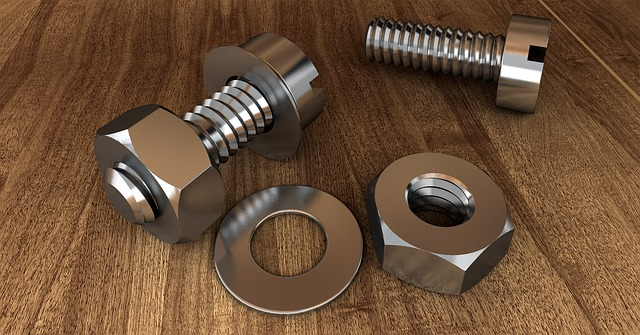
\includegraphics[width=\linewidth]{screw-1924174_640.jpg} % Figure image
	\caption{Nuts n Bolts} % Figure caption
	\label{screw-1924174_640} % Label for referencing with \ref{bear}
\end{figure}


\subsection{Problem Statement}
%In this section, you will want to clearly define the problem that you are trying to solve, including the strategy (outline of tasks) you will use to achieve the desired solution. You should also thoroughly discuss what the intended solution will be for this problem. Questions to ask yourself when writing this section:

%Is the problem statement clearly defined? Will the reader understand what you are expecting to solve?

%Have you thoroughly discussed how you will attempt to solve the problem?

%Is an anticipated solution clearly defined? Will the reader understand what results you are looking for?

Classifiers such as AlexNet and VGGNet which are typically trained on single class image data such as the 1000 class ImageNet dataset are also able to classify multiple objects in images even though they weren't specifically trained to do so. This happens because the output of the classifier is simply a list of probabilities for every possible class label.  These probabilities range from zero to one and the probability whose value is closest to one is typically regarded as the \textit{winning} prediction.  However, if we take the top 3 or even the top 5 highest probable labels we will often find that these \textit{runner-up} predictions can also be found in the image.  

The problem that we will try to solve is finding multiple features (or labels) in a single image. We would also like to know how much better our trained multi-label classifier is at predicting the top $k$ labels for a given image as compared to a standard single-label classifiers like VGG16~\cite{SimonyanZ14a} trained on ImageNet? Can we train a classifier using multi-labeled image data to perform at least as well as existing models trained on single-class image data.  A model trained on multi-labeled image data should, in theory, require fewer data samples since more information per image is available to training. Is this also true?  Let's find out.


\subsection{Metrics}\label{sec:metrics}

\begin{figure*}[!t]
\normalsize
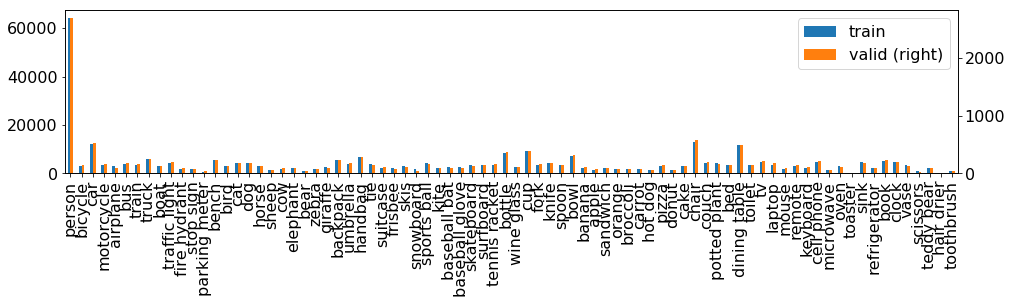
\includegraphics[width=\linewidth]{mscoco_label_counts.png}
\caption{Number of samples in MS-COCO containing at least one instance of a label.}
\label{fig:coco_label_counts}
\vspace*{4pt}
\end{figure*}

%In this section, you will need to clearly define the metrics or calculations you will use to measure performance of a model or result in your project. These calculations and metrics should be justified based on the characteristics of the problem and problem domain. Questions to ask yourself when writing this section:

%Are the metrics you’ve chosen to measure the performance of your models clearly discussed and defined?
%Have you provided reasonable justification for the metrics chosen based on the problem and solution?

After reading through previous literature on multi-label classification, we found that there are quite a few metrics appropriate for this problem. The mean average precision (mAP) is a widely used metric for comparing between trained models and has been regarded as the best metric for classification problems~\cite{Lavrenko_2014}.  Other popular metrics include precision, recall, $F_1$ score, Jaccard index, 0/1 loss and Hamming loss~\cite{Tsoumakas:2007,SOKOLOVA2009427,Herrera:2016}. 

For multi-label classification, particularly, the precision, recall, and $F_1$ score have three different variants which we will use~\cite{MADJAROV20123084,WuZ16,Koyejo:2015,GongJLTI13}. \textit{Macro-averaging} measures the average classification performance across labels.  

\begin{equation}
\mathrm{MP} = \frac{1}{L}\sum_{j=1}^{L}\frac{\sum_{i=1}^{N}y_{ij}\hat{y}_{ij}}{\sum_{i=1}^{N}y_{ij}}
\label{eq:MP}
\end{equation}

\begin{equation}
\mathrm{MR} = \frac{1}{L}\sum_{j=1}^{L}\frac{\sum_{i=1}^{N}y_{ij}\hat{y}_{ij}}{\sum_{i=1}^{N}\hat{y}_{ij}}
\label{eq:MR}
\end{equation}

\begin{equation}
\mathrm{MF_1} = \frac{1}{L}\sum_{j=1}^{L}\frac{2\sum_{i=1}^{N}y_{ij}\hat{y}_{ij}}{\sum_{i=1}^{N}\hat{y}_{ij}+\sum_{i=1}^{N}y_{ij}}
\label{eq:MF1}
\end{equation}

This metric treats all classes equal regardless of their sample size, so focusing on getting rare classes right can result in a significant increase in performance. To counterbalance this bias we also perform \textit{instance-averaging} which measures average classification performance across examples,

\begin{equation}
\mathrm{iP} = \frac{1}{N}\sum_{i=1}^{N}\frac{\sum_{j=1}^{L}y_{ij}\hat{y}_{ij}}{\sum_{j=1}^{L}y_{ij}}
\label{eq:iP}
\end{equation}

\begin{equation}
\mathrm{iR} = \frac{1}{N}\sum_{i=1}^{N}\frac{\sum_{j=1}^{L}y_{ij}\hat{y}_{ij}}{\sum_{j=1}^{L}\hat{y}_{ij}}
\label{eq:iR}
\end{equation}

\begin{equation}
\mathrm{iF_1} = \frac{1}{N}\sum_{i=1}^{N}\frac{2\sum_{j=1}^{L}y_{ij}\hat{y}_{ij}}{\sum_{j=1}^{L}\hat{y}_{ij}+\sum_{j=1}^{L}y_{ij}}
\label{eq:iF1}
\end{equation}

and \textit{micro-averaging} which measures average classification performance across both labels and samples.

\begin{equation}
\mathrm{\mu P} = \frac{\sum_{i=1}^{N}\sum_{j=1}^{L}y_{ij}\hat{y}_{ij}}{\sum_{i=1}^{N}\sum_{j=1}^{L}y_{ij}}
\label{eq:mP}
\end{equation}

\begin{equation}
\mathrm{\mu R} = \frac{\sum_{i=1}^{N}\sum_{j=1}^{L}y_{ij}\hat{y}_{ij}}{\sum_{i=1}^{N}\sum_{j=1}^{L}\hat{y}_{ij}}
\label{eq:mR}
\end{equation}

\begin{equation}
\mathrm{\mu F_1} = \frac{2\sum_{i=1}^{N}\sum_{j=1}^{L}y_{ij}\hat{y}_{ij}}{\sum_{i=1}^{N}\sum_{j=1}^{L}\hat{y}_{ij}+\sum_{i=1}^{N}\sum_{j=1}^{L}y_{ij}}
\label{eq:mF1}
\end{equation}

For both of these, the more frequent classes will be dominant and have a greater impact on performance.

Equations~\ref{eq:MP} through~\ref{eq:mF1} require the $\hat{y}_{ij}$ values to be binary 1/0 predictions.  However, most classifier models including ours return an output of predictions in the form of floating point values on the interval $[0,1]$. The process of turning these raw predictions into binary predictions is commonly referred to as \textit{label decision} and there are two common approaches to this type of decision: top-$k$ and thresholding.~\cite{Li2017a}

%\begin{figure*}[!t]
%\normalsize
%\begin{equation}
%\label{eqn_dbl_x}
%x = 5 + 7 + 9 + 11 + 13 + 15 + 17 + 19 + 21+ 23 + 25 + 27 + 29 + 31
%\end{equation}
%\begin{equation}
%\label{eq:wideeq}
%{\cal R}^{(\text{d})}=
% g_{\sigma_2}^e
% \left(
%   \frac{[\Gamma^Z(3,21)]_{\sigma_1}}{Q_{12}^2-M_W^2}
%  +\frac{[\Gamma^Z(13,2)]_{\sigma_1}}{Q_{13}^2-M_W^2}
% \right)
% + x_WQ_e
% \left(
%   \frac{[\Gamma^\gamma(3,21)]_{\sigma_1}}{Q_{12}^2-M_W^2}
%  +\frac{[\Gamma^\gamma(13,2)]_{\sigma_1}}{Q_{13}^2-M_W^2}
% \right)\;.
%\end{equation}
%\begin{equation}
%\label{eqn_dbl_y}
%y = 4 + 6 + 8 + 10 + 12 + 14 + 16 + 18 + 20+ 22 + 24 + 26 + 28 + 30
%\end{equation}
%\hrulefill
%\vspace*{4pt}
%\end{figure*}

In the top-$k$ approach, for each sample, the $k$ labels with the highest prediction value are set to 1 and the rest are set to 0.  This approach works very well when working with datasets that have nice evenly distributed labels across samples but less so when working with unbalanced datasets. One variation of the top-$k$ approach is to use a \textit{per-sample} top-$k$, the value of which is determined by the number of ground truth labels in each sample.  For example, if a sample has 3 ground truth labels, then we assign a 1 to the top 3 predictions from that sample and 0 to the rest of the predictions.  The next sample might only have 1 ground truth label in which case only the highest predicted value will be set to 1.  And so on for the rest of the dataset.  We have not yet seen this approach in the literature but think it might be interesting to investigate.

The second type of label decision is thresholding. Using this approach the label is predicted as present if the raw prediction exceeds some predefined threshold $\tau$. 
\begin{equation}
\hat{y}_{ij} = \left\{
    \begin{array}{lll}
        1 & \mathrm{if} & h_{ij} \geq \tau \\
        0 & \mathrm{if} & h_{ij} < \tau
    \end{array}
\right.
\end{equation}
Typically this value is set to 0.5 and is a logical choice for multi-class classification where the raw predictions come from the output of a softmax layer.  For multi-label classification it is more common to see a sigmoid function used for the final layer, hence the separation between positive and negative predictions becomes less obvious. To this end, we choose a threshold that minimizes the difference in label cardinality between the ground truth labels $y_{ij}$ and the predictions $\hat{y}_{ij}$.~\cite{Read:2011}

\begin{equation}
\mathrm{LCard} = \frac{1}{N}\sum_{i=1}^{N}\sum_{j=1}^{L}y_{ij}
\label{eq:lcard}
\end{equation}

\begin{equation}
\tau = \mathrm{argmin}\left\|\left(\mathrm{LCard}-\frac{1}{N}\sum_{i=1}^{N}\sum_{j=1}^{L}1_{h_{ij} \geq \tau}\right)\right\|
\label{eq:tau}
\end{equation}
When comparing our model to the benchmark models, we will use Eqns.~\ref{eq:MP} through~\ref{eq:mF1}. When comparing the results of our model to those previously reported in the literature, we will restrict ourselves to using only those metrics for which there is a direct comparison to the previous work.

%The Mean Average Precision @ 5 is:
%\begin{equation}
%MAP@5 = \frac{1}{|U|}\sum_{u=1}^{|U|}\sum_{k=1}^{min(5,n)}P(k)
%\label{eq:map5}
%\end{equation}
%where $|U|$ is the number of user events, $P(k)$ is the precision at cutoff $k$, $n$ is the number of predicted clusters.

\section{Analysis} % approx. 2-4 pages
\subsection{Data Exploration}
%In this section, you will be expected to analyze the data you are using for the problem. This data can either be in the form of a dataset (or datasets), input data (or input files), or even an environment. The type of data should be thoroughly described and, if possible, have basic statistics and information presented (such as discussion of input features or defining characteristics about the input or environment). Any abnormalities or interesting qualities about the data that may need to be addressed have been identified (such as features that need to be transformed or the possibility of outliers). Questions to ask yourself when writing this section:

%We use the NUS-WIDE\cite{nus-wide-civr09} dataset as our secondary dataset.
%If a dataset is present for this problem, have you thoroughly discussed certain features about the dataset? 
%Has a data sample been provided to the reader?
%If a dataset is present for this problem, are statistics about the dataset calculated and reported? 
%Have any relevant results from this calculation been discussed?
%If a dataset is **not** present for this problem, has discussion been made about the input space or input data for your problem?
%Are there any abnormalities or characteristics about the input space or dataset that need to be addressed? (categorical variables, missing values, outliers, etc.)


For this study we will use the (2017) MS-COCO\cite{MSCOCO} dataset as our primary dataset. The COCO dataset is freely downloadable from the internet and contains images with multiple labels per image making them ideal for this kind of study. The COCO dataset contains a training set of 118,287 images and a validation set of 5,000 images.  The images are colored and the size of each image is about 600 * 400 pixels.  The MS-COCO dataset has 80 labels with 2.9 labels per image on average.  However, both training and validation sets have images with no labels.  This is not so much a problem for training as it is for testing.  Specifically, when we evaluate our predictions using the metrics from Section~\ref{sec:metrics}, empty labeled samples could lead to divide by zero errors.  Hence, we will only use labeled samples for testing. 

%They are also large enough that we can use them for training.

%Both datasets are feely downloadable from the internet.  However, we had to explicitly request permission to use and download the image set for the NUS-WIDE dataset.  The authors were happy to grant us permission.

%The NUS-WIDE dataset contains 269,648 images and 81 labels with 2.4 labels per image on average.  The images vary in size (height and width values fall within the range between about 150 pixels to 250 pixels) and shape (portrait and landscape) and all have 3 color channels. We will use the original train/test split of 161,789 and 107,859. 

%Since we will be fine-tuning a model pretrained on ImageNet, these two datasets are good candidates since all their labels are a subset of the original 1000 ImageNet labels.

%coco
%        train, valid
%2017   118287,  5000
%2015
%2014

%nus-wide
%         train ,   test
%Object   17928 ,  12072
%Scene    17463 ,  17463
%Lite     27807 ,  27808
%All     161789 , 107859


%images in Lite train, valid, test, dataset have missing tags.
%test
%before (13904, 224, 224, 3) (13904, 81)
%after  (13160, 224, 224, 3) (13160, 81)

%TrainTestLabels/Labels_lake_Train.txt line 78373 value = -1130179

%All
%\begin{table}
%\begin{tabular}{rrrr}
%\toprule
%{} &   test &  train &  valid \\
%\midrule
%0  &  12006 &  36340 &  11955 \\
%1  &  15780 &  47571 &  15865 \\
%2  &  10531 &  31614 &  10499 \\
%3  &   6652 &  19747 &   6665 \\
%4  &   4151 &  12304 &   4149 \\
%5  &   2429 &   7283 &   2495 \\
%6  &   1374 &   3989 &   1360 \\
%7  &    667 &   1969 &    627 \\
%8  &    250 &    730 &    233 \\
%9  &     70 &    190 &     63 \\
%10 &     15 &     46 &     15 \\
%11 &      4 &      3 &      3 \\
%12 &      0 &      2 &      0 \\
%13 &      1 &      0 &      0 \\
%\bottomrule
%\end{tabular}
%\end{table}

%Lite
%\begin{table}
%\begin{tabular}{rrrr}
%\toprule
%{} &  test &  train &  valid \\
%\midrule
%0  &   744 &   1474 &    771 \\
%1  &   963 &   1971 &    996 \\
%2  &   685 &   1292 &    709 \\
%3  &   414 &    742 &    431 \\
%4  &  5109 &  10344 &   5152 \\
%5  &  3092 &   6143 &   2972 \\
%6  &  1680 &   3385 &   1658 \\
%7  &   819 &   1632 &    812 \\
%8  &   296 &    617 &    300 \\
%9  &    82 &    161 &     80 \\
%10 &    15 &     40 &     21 \\
%11 &     5 &      3 &      2 \\
%12 &     0 &      2 &      0 \\
%13 &     0 &      1 &      0 \\
%\bottomrule
%\end{tabular}
%\end{table}

%Object
%\begin{table}
%\begin{tabular}{rrrr}
%\toprule
%{} &  test &  train &  valid \\
%\midrule
%0 &     0 &      0 &      0 \\
%1 &  4861 &  14270 &   4822 \\
%2 &  1135 &   3535 &   1171 \\
%3 &    40 &    122 &     42 \\
%4 &     0 &      1 &      1 \\
%\bottomrule
%\end{tabular}
%\end{table}

%Scene
%\begin{table}
%\begin{tabular}{rrrr}
%\toprule
%{} &  test &  train &  valid \\
%\midrule
%0  &   396 &    877 &    427 \\
%1  &   985 &   2073 &   1037 \\
%2  &  1835 &   3530 &   1721 \\
%3  &  1811 &   3680 &   1790 \\
%4  &  1455 &   2892 &   1474 \\
%5  &  1108 &   2271 &   1164 \\
%6  &   719 &   1328 &    711 \\
%7  &   328 &    594 &    302 \\
%8  &    74 &    175 &     90 \\
%9  &    16 &     38 &     14 \\
%10 &     5 &      4 &      0 \\
%11 &     0 &      1 &      1 \\
%\bottomrule
%\end{tabular}
%\end{table}


\subsection{Exploratory Visualization}
%In this section, you will need to provide some form of visualization that summarizes or extracts a relevant characteristic or feature about the data. The visualization should adequately support the data being used. Discuss why this visualization was chosen and how it is relevant. Questions to ask yourself when writing this section:

%Have you visualized a relevant characteristic or feature about the dataset or input data?
%Is the visualization thoroughly analyzed and discussed?
%If a plot is provided, are the axes, title, and datum clearly defined?

\begin{figure*}[!t]
\normalsize
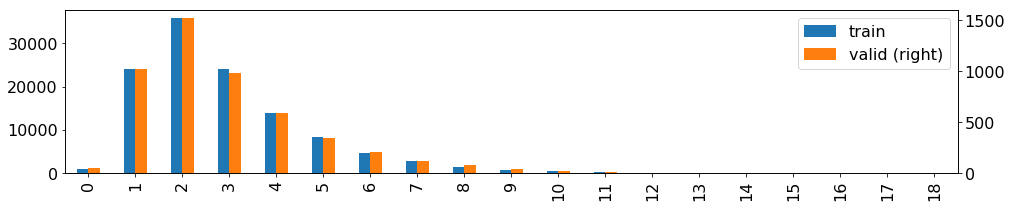
\includegraphics[width=\linewidth]{mscoco_n_images_with_k_tags.png}
\caption{Number of unique labels per sample in MS-COCO.}
\label{fig:coco_n_images_with_k_tags}
\vspace*{4pt}
\end{figure*}

In Fig.~\ref{fig:coco_label_counts}, we can see that the dominating class label is \textit{person} with 64115 occurrences in the training set and 2693 in the validation set. The least dominating class labels are the \textit{toaster} and \textit{hair drier} with 217 and 189 in the training set and 8 and 9 in the validation set, respectively.
In Fig.~\ref{fig:coco_n_images_with_k_tags}, we show the number of unique tags per sample. The majority of the samples have at least 1 to 4 unique labels with 2 unique labels being the most dominate. We also notice that the training and testing sets have 1021 and 48 samples with no labels. We will keep this fact in mind when running our evaluation metrics.
In both figures, the training set has 20 to 30 times more samples per label than the validation set and the ratios between the training and validation sets are consistent (i.e. the heights of the train and valid bars are about the same.)

\subsection{Algorithms and Techniques}\label{sec:algo}
%In this section, you will need to discuss the algorithms and techniques you intend to use for solving the problem. You should justify the use of each one based on the characteristics of the problem and the problem domain. Questions to ask yourself when writing this section:

%Are the algorithms you will use, including any default variables/parameters in the project clearly defined?
%Are the techniques to be used thoroughly discussed and justified?
%Is it made clear how the input data or datasets will be handled by the algorithms and techniques chosen?

To solve this problem, we will model our classifier using a deep convolutional neural net. We will not train our model from scratch, but rather we will perform transfer learning using the VGG16 convnet trained on ImageNet. We will read the images from disk and perform data augmentation using worker threads. This will make it so the GPU doesn't have to wait on batches thereby maximizing our training efficiency. We will use sigmoid activation in the output layer~\cite{Kurata:2016}, binary cross entropy for our loss function~\cite{deBoer2005} and mini-batch stochastic gradient descent with momentum for backpropogation. Table~\ref{tab:hyperparams} outlines the hyper-parameters that will be tuned to optimize the classifier.
\begin{table}
\caption{List of hyper-parameters to tune to optimize the classifier. There are 2 options for image preprocessing that is used by both Stage 1 and 2: inet - use a global scaling factor and zmuv - use per-image zero-mean unit-variance.  Stage 1 is where the top model gets trained with bottleneck features.
%BN stands for Batch Normalization.
We train the entire model (base + top) in Stage 2.  Please refer to Sec.~\ref{sec:method} for more details. Note: Batch sizes of 256 will be used only for a few select cases.}
\label{tab:hyperparams}
\centering
\begin{tabular}{cll}
\toprule
%\hline
Stage & Hyper-parameter & Variants \\
\midrule
%\hline
 & Image Preprocessing & INET, ZMUV \\
\midrule
%\hline
1 & Classifier Design & 77, avg, max \\
1 & Number of Hidden FC Layers & 1 or 2 \\
1 & Number of Nodes per Layer & 1024, 2048, 4096 \\
%1 & Regularization Method & BN or Dropout \\
1 & Learning Rate & 0.1, 0.05\\
1 & Batch Size & 32, 64, 128, 256\\
\midrule
%\hline
2 & Number of Frozen Layers & 15, All \\
2 & Learning Rate & \\
2 & Batch Size & 32, 64, 128, 256 \\
2 & Data Augmentation & h, w, r, s, z, f \\
\bottomrule
%\hline
\end{tabular}
\end{table}
We will also use some Keras callbacks during our training.  ModelCheckpoint to save only the best models at each epoch, EarlyStopping to stop training when we stop making progress and CSVLogger for plotting purposes.


\subsection{Benchmark}
%In this section, you will need to provide a clearly defined benchmark result or threshold for comparing across performances obtained by your solution. The reasoning behind the benchmark (in the case where it is not an established result) should be discussed. Questions to ask yourself when writing this section:

%Has some result or value been provided that acts as a benchmark for measuring performance?
%Is it clear how this result or value was obtained (whether by data or by hypothesis)?

We were unable to find a VGG16 model trained on COCO to use for benchmarking purposes.  But we did find multiple results of multi-label classifiers trained on COCO in the literature.  We will use these results when evaluating the performance of our model in~\ref{sec:eval}.

\section{Methodology}\label{sec:method} % approx. 3-5 pages
\subsection{Data Preprocessing}\label{sec:preproc}
%In this section, all of your preprocessing steps will need to be clearly documented, if any were necessary. From the previous section, any of the abnormalities or characteristics that you identified about the dataset will be addressed and corrected here. Questions to ask yourself when writing this section:

%If the algorithms chosen require preprocessing steps like feature selection or feature transformations, have they been properly documented?
%Based on the **Data Exploration** section, if there were abnormalities or characteristics that needed to be addressed, have they been properly corrected?
%If no preprocessing is needed, has it been made clear why?

There are 2 types of preprocessing we do on the image data. The first is image resizing and normalizing. Before passing any image through the network it must first be resized to match the height and width of the input layer and its values must be converted (normalized) from uint8's to float32's in the range of -1 and 1.  The method by which the images are normalized became a tunable hyper-parameter.  Keras comes shipped with a preprocess\_image\footnote{\url{https://github.com/keras-team/keras/blob/master/keras/applications/ImageNet_utils.py}} function that is intended to be used for data normalization on VGG16.  If using Keras with the Tensorflow backend this normalization boils down to dividing by 127.5 and then subtracting by 1 for every image.  This is the INET option in Table~\ref{tab:hyperparams}. As an alternate option, the various flavors of model generators in Keras provide to option to normalize images by either featurewise or samplewise zero-mean unit-variance (or ZMUV).  These three normalization methods each provide slightly different results and so we leave the decision as to which one is best as a tunable hyper-parameter.\footnote{This part of the study raised an interesting question. Should the input image normalization method be part of the (or be supplied as) supplemental information to the saved model?  In other words, if I download and use a trained model, should I not also expect the model to somehow tell me in what format the model expects the input data to be? There seemed to be conflicting opinions as to which normalizing method should be used.}

The other type of image preprocessing involves various forms of data augmentation.  Going by the codes in Table~\ref{tab:hyperparams} we will augment the image data by (h) shifting along the height direction, (w) shift along the width direction, (r) performing random rotation, (s) skew transform, (z) multiplying by a zoom factor, and (f) performing horizontal flips.  We will also shuffle the training data after each epoch. We will only perform data augmentation during training, not during top model training as the input images to the top model aren't images but rather features of a deep layer.

\subsection{Implementation}
%In this section, the process for which metrics, algorithms, and techniques that you implemented for the given data will need to be clearly documented. It should be abundantly clear how the implementation was carried out, and discussion should be made regarding any complications that occurred during this process. Questions to ask yourself when writing this section:

%Is it made clear how the algorithms and techniques were implemented with the given datasets or input data?
%Were there any complications with the original metrics or techniques that required changing prior to acquiring a solution?
%Was there any part of the coding process (e.g., writing complicated functions) that should be documented?

The implementation is divided into 2 stages. In the first stage we load the VGG16 model but without the last 3 fully connected layers. These layers are specific to the 1000 ImageNet classes that the VGG16 model was originally trained on. We then run a single prediction calculation the both the training and validation sets. But instead of getting the typical label predictions, we get the output of the last VGG16 convolutional layer. Depending on our Classifier Design (See Table~\ref{tab:hyperparams}), the output will either be (77) the raw $7\times7\times512$ features, (avg) the 512 features that result from applying global average pooling to the raw features, or (max) the 512 features that result from applying global max pooling to the raw features. We refer to these as bottleneck features and save them (along with their ground truth labels) as python numpy arrays. We then construct a small\footnote{Small in comparison to the base VGG16 model which is 16 layers deep. Our classifier will have a single hidden layer between the input layer and the output layer.} classifier model that we can train using the bottleneck features. The goal of Stage 1 is to train this "top" model as best we can before attaching it to the VGG16 base for fine tuning. There are a few reasons for pretraining the classifier. The top model has fewer layers and the bottleneck features are much smaller $7\times7\times512=25088$ than the original raw images $224\times224\times3=150528$. This leads to fewer parameters to learn and faster training. We will still need to fine tune the full model in Stage 2, but pretraining the top model in this way provides a much better starting guess than simply initializing the top model with random weights. Another happy side effect of pretraining the classifier is we can make faster progress with tuning many of our hyper-parameters. Specifically, the optimal classifier design, regularization method, and number of nodes per layer can each be found much faster.

\begin{figure*}%[!t]
\normalsize
\subfloat[][]{
\label{fig:top_pp_pl_lve}
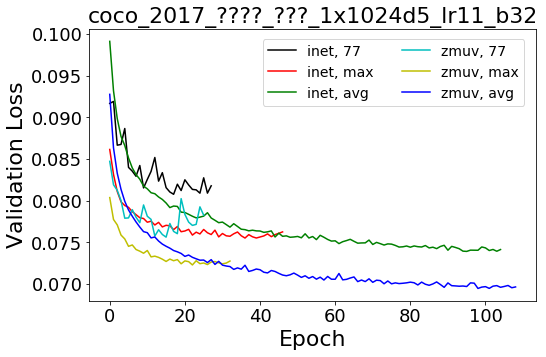
\includegraphics[width=0.49\linewidth]{top_pp_pl_loss_vs_epoch.png}}
\subfloat[][]{
\label{fig:top_pl_sz_lve}
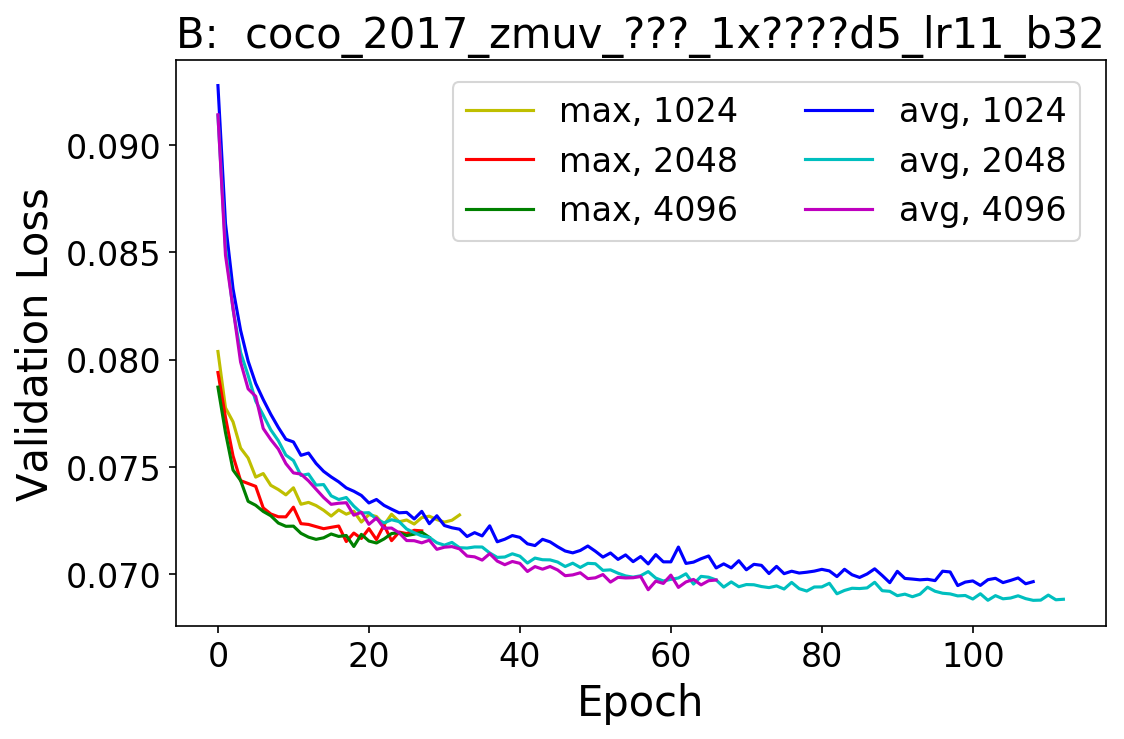
\includegraphics[width=0.49\linewidth]{top_pl_sz_loss_vs_epoch.png}}
\caption{Top model validation losses as a function of epoch. Each panel explores a different set of hyper-parameters. The yellow and blue curves are of the same data in both plots.}
\label{fig:top1_pp_pl_sz}
\vspace*{1pt}
\end{figure*}

Once the optimal Stage 1 hyper-parameters are found then we can proceed to Stage 2 and attach our freshly trained classifier to our base VGG16 model. We can choose to freeze a certain number of layers (in the base model) before we start fine tuning or we can freeze them all. For this project we either freeze all layers or just the ones up to the last convolutional block. Weights on frozen layers do not update during backpropogation. Since we are now training the final model on the raw images it's safe to augment our data as prescribed in Section~\ref{sec:preproc}. We vary the learning rate for various batch sizes as presented in Table~\ref{tab:hyperparams} and choose the model which minimizes the loss function. 

\subsection{Refinement}\label{refine}

%In this section, you will need to discuss the process of improvement you made upon the algorithms and techniques you used in your implementation. For example, adjusting parameters for certain models to acquire improved solutions would fall under the refinement category. Your initial and final solutions should be reported, as well as any significant intermediate results as necessary. Questions to ask yourself when writing this section:

%Has an initial solution been found and clearly reported?
%Is the process of improvement clearly documented, such as what techniques were used?
%Are intermediate and final solutions clearly reported as the process is improved?

At this point we would like to refine our model by tuning some of the Stage 1 hyper-parameters.  We begin by defining some rules for how we will format our log and top model weights filenames\footnote{Logs will be saved as csv's and the weights will be saved in hdf format using the hdf5 extension. The files can be found from the root of the project directory in data/bottleneck\_top\_models.}. This is best explained with a simple example. Consider the following string, "coco\_2017\_zmuv\_avg\_1x2048d5\_lr11\_b32". The first field, "coco", refers to the name of the dataset and "2017" is the subset (or version) of the dataset. The other fields follow directly from Table~\ref{tab:hyperparams}. "ZMUV" indicates zero-mean unit-variance scaling was used to normalize the input images. The $4^{th}$ field, "avg" denotes the use of global average pooling on the final layer of the base VGG16 model. This also describes the shape of the input to the top model. The next term, "1x2048d5" is a combination of 3 hyper-parameters that describe the fully connected layers in the top model. The "1x2048" indicates that there is 1 hidden layer and that it has "2048" nodes.  All fully connected layers are immediately followed by a ReLU activation layer which is then followed by either a dropout ("d") layer or a batch normalization ("bn") layer. For dropout, the number after the "d" indicates the percentage of nodes that get dropped. So "d3" would mean that only 30\% of the nodes are dropped. The second to last field gives information about the learning rate in the form "lrXY" which should be interpreted as $\mathrm{lr = X * 10^{-Y}}$.  So, lr53 would indicate a learning rate of 0.005, lr11 would be 0.1, and so forth. The final field, "b32" denotes the batch size.

The first hyper-parameter we looked at was the method for image preprocessing. We compared the results between each method by looking at how they compared for each of the different classifier designs. In all cases, the ZMUV preprocessing method led to lower validation losses as seen in Fig.~\ref{fig:top_pp_pl_lve}. We also looked at how well the different classifier designs compared to each other. Looking again at Fig.~\ref{fig:top_pp_pl_lve} we can see that the 77 design performed much worse than the global max and global average pooling designs. To determine whether global max or global average pooling is better, we compare them against different layer sizes as shown in Fig.~\ref{fig:top_pl_sz_lve}. In all three cases the validation loss was lower when using global average pooling. In light of these preliminary results we will restrict the remaining hyper-parameter tuning calculations to using only ZMUV to preprocess the images and global average pooling to cap off the end of the VGG16 pretrained model. A consequence of transfer learning is that the input shape of our top model will need to match the output shape of our base model. With global average pooling, this simplifies the input shape from $512\times7\times7$ features to $512\times1\times1$ features. This will greatly reduce the training time of our top model classifier and enable faster progress while we tune the remaining hyper-parameters.

\begin{figure}%[!ht]
\normalsize
\subfloat[][]{
\label{fig:top_nl_sz_lve}
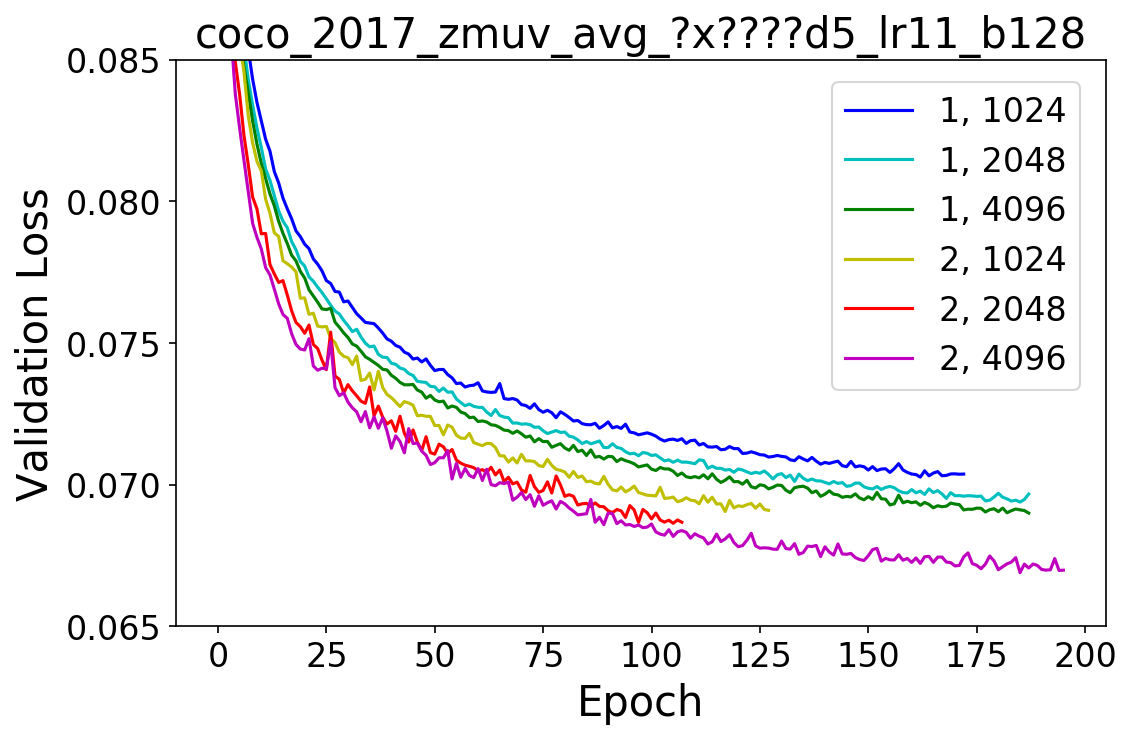
\includegraphics[width=\linewidth]{top_nl_sz_loss_vs_epoch}} \\
\subfloat[][]{
\label{fig:top_nl_lr_lve}
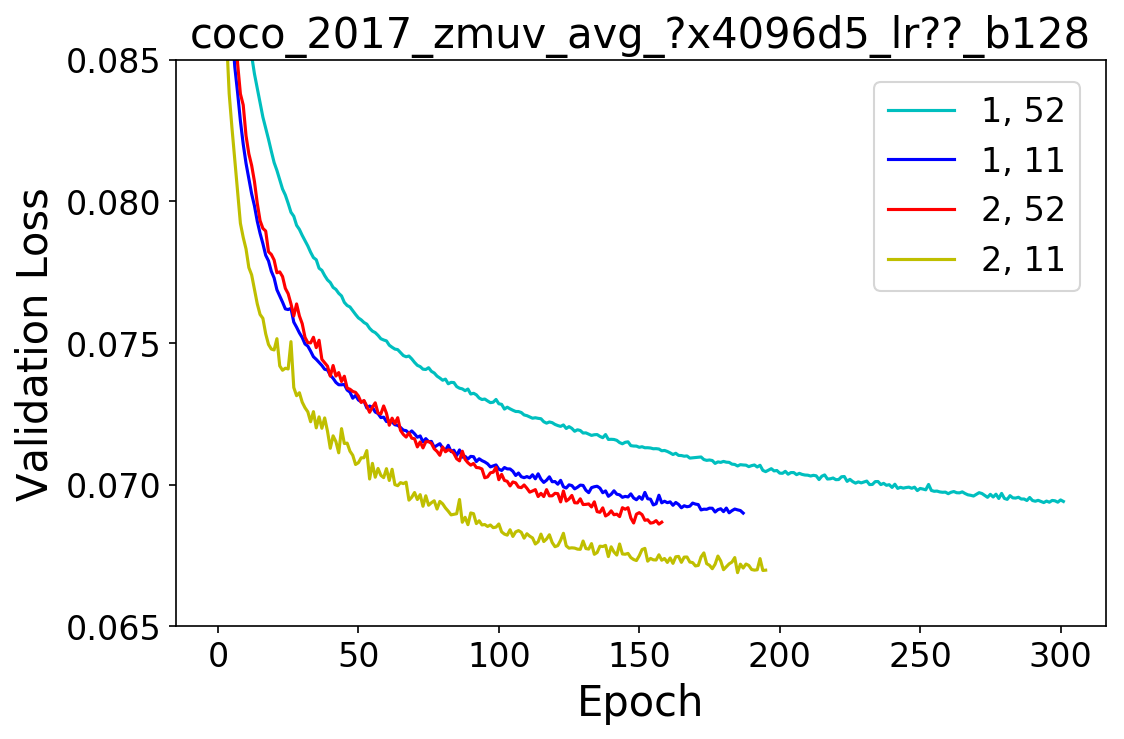
\includegraphics[width=\linewidth]{top_nl_lr_loss_vs_epoch}} \\
\subfloat[][]{
\label{fig:top_sz_lr_lve}
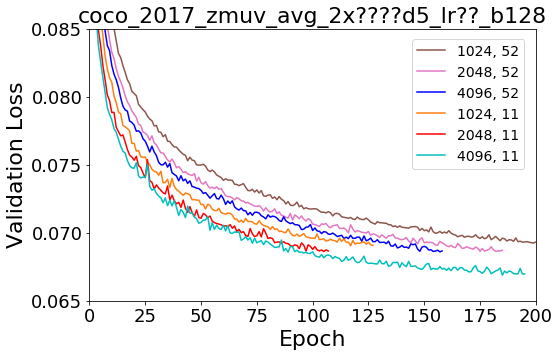
\includegraphics[width=\linewidth]{top_sz_lr_loss_vs_epoch}} \\
\caption{Top model validation losses as a function of epoch. Each panel explores a different set of hyper-parameters. All results are for a mini batch size of 128. The colors are the same for same data in each plot.  For example, The teal curves in all three plots are of the same data. The shorter curves are a result of early stopping. Refer to Section~\ref{refine} for further details.}
\label{fig:top2_nl_sz_lr}
\vspace*{1pt}
\end{figure}

The results of Fig.~\ref{fig:top_pl_sz_lve} also suggest that there may exist a relationship between the validation loss and the layer size, namely that increasing the number of nodes per layer brings about lower validation losses. It worth noting that up until now we have been using a somewhat high learning rate of 0.1. The higher the learning rate the more the validation loss fluctuates from one training epoch to the next. This fact makes it hard to say one way or another which layer size is better. 

\begin{figure*}%[!t]
\subfloat[][]{
\normalsize
\label{fig:top_lr_bs_lve}
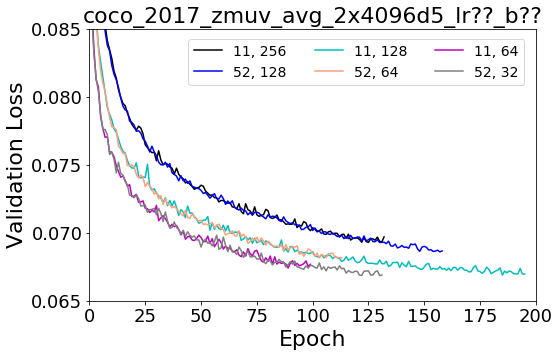
\includegraphics[width=0.49\linewidth]{top_lr_bs_loss_vs_epoch.png}}
\subfloat[][]{
\normalsize
\label{fig:top_lr_bs_lvt}
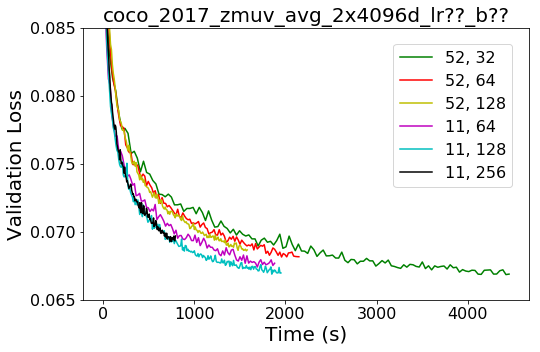
\includegraphics[width=0.49\linewidth]{top_lr_bs_loss_vs_time.png}}
\caption{Top model validation losses as a function of (a) epoch and (b) time. The lr11 and lr52 correspond to 0.1 and 0.05 learning rates respectively.  In (b), We scaled the x-axis for each run by multiplying through the average training time per epoch. The colors of the curves are matched up to help guide the eye.}
\label{fig:top3_lr_bs}
\vspace*{1pt}
\end{figure*}

In the rest of this section, we present the results from a grid search that we performed on the remaining top model hyper-parameters, namely those listed under Table~\ref{tab:hyperparams} stage 1. The original VGG16 model has 3 dense fully connected layers. The first 2 layers are hidden and have 4096 nodes each. The last output layer has 1000 nodes equal to the number of classes in ImageNet. Since the COCO dataset consists of only 80 unique classes we will test the performance of using only a single hidden layer and compare it to that when we use 2 hidden layers. We would also like to see how different layer sizes (1024, 2048, and 4096) affect performance. The default size of the hidden layers in VGG16 is 4096. Again, since we are working with only 80 classes, we may be able to get as good performance with smaller layer sizes. As we did before in Fig.~\ref{fig:top1_pp_pl_sz} we will use a learning rate of 0.1 but also compare how the performance changes when we cut the learning rate in half (e.g. 0.05). In general, the higher the learning rate, the faster the training time. If it appears from these preliminary results that we need to explore further smaller learning rates, we will do so on a case by case basis. The final hyper-parameter for tuning our top model is the batch size. We will look at 3 sizes, 32, 64, 128, and on a few rare cases 256. The grid search on these four hyper-parameters yields $2*3*2*3 = 32$ pretraining runs. For brevity, only a selection of these results are shown\footnote{See the Jupyter notebook for all 32 pretraining plots.}. 

The results shown of Fig.~\ref{fig:top2_nl_sz_lr} are all for a mini batch size of 128. In Fig.~\ref{fig:top_nl_sz_lve}, we compare how the number of hidden layers and the size of the hidden layers affects performance. For both the single and double layer cases validation loss decreases with increased layer size. Also, the losses for the double layer models are all lower than those of the single layer models. Next, in Fig.~\ref{fig:top_nl_lr_lve}, we hold the layer size fixed at 4096 nodes per layer and compare relationships between the number of layers and the learning rate. Independent of the learning rate, the double hidden layer runs perform much better than the single hidden layer runs. We also observe that the training runs with the higher learning rate start to flatten out a little faster than the others. This is typical as higher learning rates tend to find a local minimum quickly. In Fig.~\ref{fig:top_sz_lr_lve}, we hold the number of hidden layers fixed at 2 layers and compare the relationship between number of nodes per layer and learning rate. As the number of nodes per layer increases the validation loss decreases. The validation loss was also lower in all cases where the larger learning rate was used. 

These results suggest better performance should be expected using 2 hidden layers with 4096 nodes per layer. Also, we can afford to use a little higher learning rate than we usually would. Typically, high learning rates tend to lead to overfitting. However, since the entropic capacity of the top model classifier is fairly low it does not have as strong a tendency to overfit.

The final hyper-parameter to optimize is the batch size. Using the results above, we set the number of layers to 2 and the number of nodes per layer to 4096. We plot the relationship between learning rate and batch size in Fig.~\ref{fig:top3_lr_bs}. In Fig.~\ref{fig:top_lr_bs_lve}, we see an interesting relationship.  The curves of training runs tend to overlap when both the learning rate and the batch size are both multiplied by the same constant factor (here 2 or $\nicefrac{1}{2}$ depending on your perspective). The loss curves in Fig.~\ref{fig:top_lr_bs_lvt} are the same as those in Fig.~\ref{fig:top_lr_bs_lve} but plotted with respect to training time. From this perspective it appears that in order to train fast one needs only focus on setting the learning rate as high as possible without overfitting. Increasing the batch size can help smooth out the validation losses between epochs and consequently reduce overfitting.

%data plots are slightly smoother for lower learning rate

It is not clear at this point what will be the best choice for our final model in terms of learning rate and batch size. In the next section we fine-tune a few different models and compare the results using our evaluation metrics. 

%coco_2017_zmuv_avg_1x1024d5_lr13_b04 148s
%coco_2017_zmuv_avg_1x1024d5_lr13_b32 20s
%coco_2017_zmuv_avg_1x1024d5_lr11_b16 44s

%coco_2017_inet_avg_1x1024d5_lr11_b32 19s
%coco_2017_inet_max_1x1024d5_lr11_b32 17s - 18s
%coco_2017_inet_77_1x1024d5_lr11_b32 51s
%coco_2017_zmuv_77_1x1024d5_lr11_b32 50s
%coco_2017_zmuv_77_1x2048bn_lr13_b128 37s
%coco_2017_zmuv_77_1x2048bn_lr52_b128 35s
%coco_2017_zmuv_77_1x4096d5_lr11_b16 222s
%coco_2017_zmuv_max_1x4096d5_lr11_b32 20s
%coco_2017_zmuv_max_1x2048d5_lr11_b32 18s

%coco_2017_zmuv_avg_1x2048bn_lr11_b16 50s
%coco_2017_zmuv_avg_1x2048bn_lr11_b32 25s
%coco_2017_zmuv_avg_1x2048bn_lr12_b32 25s
%coco_2017_zmuv_avg_1x2048bn_lr12_b64 13s
%coco_2017_zmuv_avg_1x2048bn_lr13_b64 13s
%coco_2017_zmuv_avg_1x2048bn_lr53_b64 13s
%coco_2017_zmuv_avg_1x2048bn_lr12_b64_15_lr12_b64_f 490s


%coco_2017_zmuv_avg_1x1024d5_lr11_b16 36
%coco_2017_zmuv_avg_1x4096d5_lr11_b16 37s - 38s
%coco_2017_zmuv_avg_2x4096d5_lr12_b128 10s
%coco_2017_zmuv_avg_2x4096d5_lr12_b32 34s
%coco_2017_zmuv_avg_2x4096d5_lr52_b256 6s
%coco_2017_zmuv_avg_3x1024d5_lr11_b32 22s
%coco_2017_zmuv_avg_3x2048d5_lr11_b32 27s
%coco_2017_zmuv_avg_3x4096d5_lr11_b32 49s


%coco_2017_zmuv_avg_1x1024d5_lr11_b32
%coco_2017_zmuv_avg_1x1024d5_lr11_b64  10s
%coco_2017_zmuv_avg_1x1024d5_lr11_b128 5s
%coco_2017_zmuv_avg_1x1024d5_lr52_b32
%coco_2017_zmuv_avg_1x1024d5_lr52_b64  9s
%coco_2017_zmuv_avg_1x1024d5_lr52_b128 4s-5s

%coco_2017_zmuv_avg_1x2048d5_lr11_b32
%coco_2017_zmuv_avg_1x2048d5_lr11_b64  9s
%coco_2017_zmuv_avg_1x2048d5_lr11_b128
%coco_2017_zmuv_avg_1x2048d5_lr52_b32 17-19s
%coco_2017_zmuv_avg_1x2048d5_lr52_b64  9s
%coco_2017_zmuv_avg_1x2048d5_lr52_b128 5s

%coco_2017_zmuv_avg_1x4096d5_lr11_b32
%coco_2017_zmuv_avg_1x4096d5_lr11_b64  10s-11s
%coco_2017_zmuv_avg_1x4096d5_lr11_b128  5s
%coco_2017_zmuv_avg_1x4096d5_lr52_b32  18-19s
%coco_2017_zmuv_avg_1x4096d5_lr52_b64   9s-10s
%coco_2017_zmuv_avg_1x4096d5_lr52_b128  5s

%coco_2017_zmuv_avg_2x1024d5_lr11_b32  21s
%coco_2017_zmuv_avg_2x1024d5_lr11_b64  10s-11s
%coco_2017_zmuv_avg_2x1024d5_lr11_b128  6s
%coco_2017_zmuv_avg_2x1024d5_lr52_b32  19-20s
%coco_2017_zmuv_avg_2x1024d5_lr52_b64  10s
%coco_2017_zmuv_avg_2x1024d5_lr52_b128  5s

%coco_2017_zmuv_avg_2x2048d5_lr11_b32  23s
%coco_2017_zmuv_avg_2x2048d5_lr11_b64  12s-13s
%coco_2017_zmuv_avg_2x2048d5_lr11_b128  7s
%coco_2017_zmuv_avg_2x2048d5_lr52_b32  24s
%coco_2017_zmuv_avg_2x2048d5_lr52_b64  11-12s
%coco_2017_zmuv_avg_2x2048d5_lr52_b128  6s

%coco_2017_zmuv_avg_2x4096d5_lr11_b32  35s
%coco_2017_zmuv_avg_2x4096d5_lr11_b64  19s
%coco_2017_zmuv_avg_2x4096d5_lr11_b128 10s
%coco_2017_zmuv_avg_2x4096d5_lr52_b32  35s
%coco_2017_zmuv_avg_2x4096d5_lr52_b64  19s
%coco_2017_zmuv_avg_2x4096d5_lr52_b128 10s


%coco_2017_zmuv_avg_1x1024d5_lr13_b04_15_lr13_b64 467s to 472s
%coco_2017_zmuv_avg_2x2048d5_lr11_b32_15_lr12_b128_hwrszf 448s
%coco_2017_zmuv_avg_2x2048d5_lr11_b32_15_lr32_b128_hwrszf 450s


\section{Results} % approx. 2-3 pages
\subsection{Model Evaluation, Validation and Justification}\label{sec:eval}
%In this section, the final model and any supporting qualities should be evaluated in detail. It should be clear how the final model was derived and why this model was chosen. In addition, some type of analysis should be used to validate the robustness of this model and its solution, such as manipulating the input data or environment to see how the model’s solution is affected (this is called sensitivity analysis). Questions to ask yourself when writing this section:

%Is the final model reasonable and aligning with solution expectations? 

%Are the final parameters of the model appropriate?
We found that the best parameters for the model were 2 hidden layers with 4096 nodes per layer.  These parameters are appropriate as they are the same as those used in the original VGG16 model.  We also experimented with different batch sizes and learning rates however we did not notice any obvious correlations to the minimal loss. The minimal losses varied between $0.06 \pm 1\times 10^{-3}$. We evaluated each of our models on precision, recall, and $\mathrm{F_1}$ score.  Based on these evaluation metrics, the 2x4096d5\_lr11\_b256\_15\_lr11\_b128\_hwrszf~\footnote{We will refer to this model as our final multi-label (FML) model from here on.} model performed the best. Interestingly, this was our 8th best model in terms of minimal loss ($L = 0.0605$). 

%Has the final model been tested with various inputs to evaluate whether the model generalizes well to unseen data?
We tested our final models against a subset of the 5000 images from the COCO 2017 validation set. The subset consisted of only those images with 1 or more labels. Images with zero labels were removed to help avoid divide-by-zero errors when calculating precision, recall, and $\mathrm{F_1}$. The final size of the test set was 4952. 

\begin{table}
\caption{Comparisons on MS-COCO validation dataset for $k=3$. The macro precision $\mathrm{MP}$, macro recall $\mathrm{MR}$, and macro $\mathrm{F}$ score $\mathrm{MF_1}$ are evaluated for each label class before averaging.  The micro precision $\mathrm{\mu P}$, micro recall $\mathrm{\mu R}$, and micro $\mathrm{F}$ score $\mathrm{\mu F_1}$ are averaged over all image-label pairs. Our final model (FML) results (2x4096d5\_lr11\_b256\_15\_lr11\_b128\_hwrszf) are provided in the bottom half of the table.}
\label{tab:PRF1}
\centering
\begin{tabular}{lllllll}
\toprule
Method & $\mathrm{MP}$ & $\mathrm{MR}$ & $\mathrm{MF_1}$ & $\mathrm{\mu P}$ & $\mathrm{\mu R}$ & $\mathrm{\mu F_1}$ \\
\midrule
KNN~\cite{nus-wide-civr09}    & 32.6 & 19.3 & 24.3 & 42.9 & 53.4 & 47.6 \\
WARP~\cite{GongJLTI13}        & 59.3 & 52.5 & 55.7 & 59.8 & 61.4 & 60.7 \\
Softmax~\cite{WangYMHHX16}    & 59.0 & 57.0 & 58.0 & 60.2 & 62.1 & 61.1 \\
BCE~\cite{WangYMHHX16}        & 59.3 & 58.6 & 58.9 & 61.7 & 65.0 & 63.3 \\
No RNN~\cite{WangYMHHX16}     & 65.3 & 54.5 & 59.3 & 68.5 & 61.3 & 65.7 \\
CNN-RNN~\cite{WangYMHHX16}    & 66.0 & 55.6 & 60.4 & 69.2 & 66.4 & 67.8 \\
ResNet-101~\cite{HeZRS15}     & 84.3 & 57.4 & 65.9 & 86.5 & 61.3 & 71.7 \\
ResNet-107~\cite{ZhuLOYW17}   & 84.4 & 57.6 & 66.1 & 86.4 & 61.4 & 71.8 \\
ResNet-101-s~\cite{ZhuLOYW17} & 84.3 & 57.7 & 66.2 & 86.3 & 61.8 & 72.0 \\
ResNet-SRNa~\cite{ZhuLOYW17} & 85.8 & 57.5 & 66.3 & 88.1 & 61.1 & 72.1 \\
ResNet-SRN~\cite{ZhuLOYW17}   & 85.2 & 58.8 & 67.4 & 87.4 & 62.5 & 72.9 \\
\midrule
best possible                 & 67.2 & 78.4 & 70.8 & 76.0 & 77.1 & 76.5 \\
\midrule % 2x4096d5_lr11_b256_15_lr11_b128_hwrszf
FML  & & & & & & \\
a. 4952 $\mathrm{(k > 0)}$       & 57.3 & 56.0 & 54.6 & 60.6 & 61.5 & 61.0 \\
%b. 4952-aug $\mathrm{(k > 0)}$   & 55.9 & 55.5 & 53.6 & 60.0 & 60.9 & 60.4 \\
b. 908 $\mathrm{(k = 3)}$       & 61.2 & 59.3 & 59.1 & 69.9 & 69.9 & 69.9 \\
c. 4952 $\mathrm{(k = L/I)}$     & 66.9 & 63.1 & 64.2 & 70.5 & 70.5 & 70.5 \\
d. 4952-a $\mathrm{(k = L/I)}$ & 65.6 & 62.9 & 63.6 & 69.8 & 69.8 & 69.8 \\
e. 4952 $\mathrm{(\tau = 0.378)}$ & 65.2 & 61.6 & 62.3 & 68.2 & 68.2 & 68.2 \\
%\midrule % 2x2048d5_lr11_b32_15_lr??_b128_hwrszf ~500s
%$\mathrm{lr = 0.001}$         & 52.7 & 52.2 & 50.5 & 58.2 & 59.1 & 58.6 \\
%$\mathrm{lr = 0.005}$         & 55.2 & 54.3 & 52.8 & 59.6 & 60.5 & 60.0 \\
%$\mathrm{lr = 0.01}$          & 56.0 & 55.6 & 53.9 & 60.1 & 61.0 & 60.6 \\
%$\mathrm{lr = 0.03}$          & 56.8 & 55.6 & 54.1 & 60.4 & 61.3 & 60.9 \\
%$\mathrm{lr = 0.05}$          & 56.7 & 55.7 & 54.1 & 60.3 & 61.3 & 60.8 \\
%\midrule % 2x4096d5_lr11_b32_15_lr??_b128_hwrszf ~450-550
%$\mathrm{lr = 0.005}$         & 55.5 & 54.6 & 53.0 & 59.7 & 60.6 & 60.1 \\
%$\mathrm{lr = 0.01}$          & 56.0 & 54.7 & 53.2 & 59.9 & 60.8 & 60.4 \\
%$\mathrm{lr = 0.05}$          & 56.1 & 55.2 & 53.7 & 59.9 & 60.8 & 60.4 \\
%\midrule % 2x4096d5_lr11_b128_15_lr52_b128_hwrszf ~442s
%5000                          & 56.8 & 56.0 & 54.5 & 60.4 & 61.1 & 60.9 \\
%2405 $\mathrm{(k >= 3)}$      & 65.2 & 45.4 & 51.4 & 75.4 & 51.5 & 61.2 \\
%908 $\mathrm{(k = 3)}$        & 59.2 & 58.5 & 57.6 & 69.4 & 69.4 & 69.4 \\
\bottomrule
\end{tabular}
\end{table}

Quantitative results on MS-COCO are presented in Table~\ref{tab:PRF1}. A summary of previous works are provided in the top portion of the table and the results from our FML model are presented in the bottom portion. Since we are dealing with a multi-label dataset, the method we use to partition the model output into true/false predictions, also known as \textit{label decision} can affect the evaluation metrics (See Section~\ref{sec:metrics}). The first set of results, FML-a, were calculated using the top-k \textit{label decision} with $k=3$ (i.e. the 3 labels with the highest prediction score).  This is a widely used method.~\cite{WangYMHHX16,ZhuLOYW17}  However, for unbalanced datasets such as COCO, this type of \textit{label decision} may not be the best choice. According to Fig.~\ref{fig:coco_n_images_with_k_tags}, only 20\% of the validation data have exactly 3 labels, 50\% of the images have less than 3 labels and 30\% have more than 3. Thus for $k=3$ it is impossible to attain perfect precision and/or recall. The best possible results are given in the table on line "best possible".  With the exception of the first two references in Table~\ref{tab:PRF1}, our FML-a results perform worse compared to all previously published results. If we evaluate the FML model strictly on the 908 images which have exactly 3 labels, our results improve substantially (See line b.) Forcing the algorithm to predict a fixed number of labels for each image does not reflect well the algorithm's performance.

\begin{figure*}%[!t]
\subfloat[][]{
\label{fig:3179}
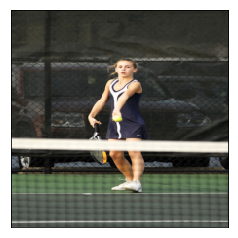
\includegraphics[width=0.195\linewidth]{coco_valid_3179.png}}
\subfloat[][]{
\label{fig:2934}
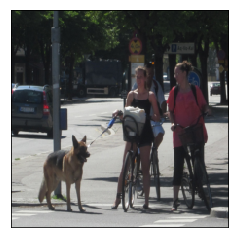
\includegraphics[width=0.195\linewidth]{coco_valid_2934.png}}
\subfloat[][]{
\label{fig:2510}
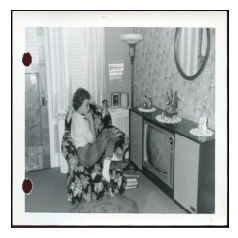
\includegraphics[width=0.195\linewidth]{coco_valid_2510.png}}
\subfloat[][]{
\label{fig:4350}
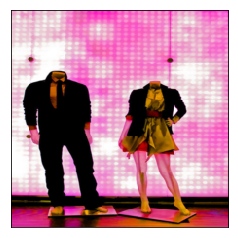
\includegraphics[width=0.195\linewidth]{coco_valid_4350.png}}
\subfloat[][]{
\label{fig:307}
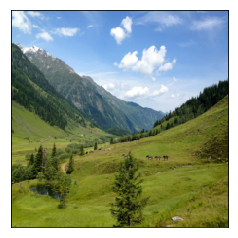
\includegraphics[width=0.195\linewidth]{coco_valid_307.png}}
\caption{Sample images from COCO. See Tables~\ref{tab:coco_valid} for corresponding predictions and ground truth.}
\label{fig:coco_valid}
\vspace*{4pt}
\end{figure*}

\begin{table*}
\caption{Ranked predictions from our model for Fig.~\ref{fig:coco_valid}. Ground truth labels are highlighted in bold.}
\label{tab:coco_valid}
\centering
\begin{tabular}{cll|cll|cll|cll|cll}
\toprule
 & Fig.~\ref{fig:3179} & pred &  & Fig.~\ref{fig:2934} & pred     &  & Fig.~\ref{fig:2510} & pred     &  & Fig.~\ref{fig:4350} & pred &  & Fig.~\ref{fig:307} & pred \\
\midrule
1 & \textbf{tennis racket} & 1.00 & 1  &   \textbf{person} & 0.98 & 1  & person & 0.99 & 1 & person & 1.00 & 1 &          sheep & 0.52 \\
2 &        \textbf{person} & 1.00 & 2  &      \textbf{car} & 0.90 & 2  &    dog & 0.57 & 5 & \textbf{tie} & 0.30 & 2 & \textbf{horse} & 0.48 \\
3 &   \textbf{sports ball} & 0.81 & 3  &      \textbf{dog} & 0.77 & 3  &           sink & 0.25 & & & & & \\
4 &           \textbf{car} & 0.02 & 4  &  \textbf{bicycle} & 0.59 & 4  &            cup & 0.24 & & & & & \\
  &                        &      & 5  &     traffic light & 0.51 & 6  & \textbf{clock} & 0.23 & & & & & \\
  &                        &      & 6  &           handbag & 0.39 & 7  & \textbf{chair} & 0.22 & & & & & \\
  &                        &      & 8  &    \textbf{truck} & 0.26 & 14 &  \textbf{book} & 0.09 & & & & & \\
  &                        &      & 10 & \textbf{backpack} & 0.24 & 20 &    \textbf{tv} & 0.07 & & & & & \\
\bottomrule
\end{tabular}
\end{table*}

One alternative to the top-k method is to instead output a variable number of labels for each image rather than a fixed number of labels for all images. An image with 5 ground truth labels would take the top-5 predictions as true whereas an image with only one ground truth label would only take the top prediction as true.  The results using this alternative method are given on line c of Table~\ref{tab:PRF1}. These results reflect better performance for our model than those previously calculated using a fixed $k$ value.

Another method commonly used to partition the model output is to use a thresholding value to split the predictions. Predictions that are greater than the thresholding value are predicted as positive. This thresholding value, $\tau$, is commonly set to $\tau = 0.5$. While this value works well for multi-class (only 1 label per image) classification where the final layer is typically a softmax layer, it does not work well for a multi-label classifier. Here our final layer is a simple sigmoid layer and as such many labels can (and should) have higher than average activations.  What we would like to do is find an optimal value of $\tau$ such that we maximize both precision and recall. Using Eqn.~\ref{eq:lcard} and~\ref{eq:tau} we calculate the optimal value of $\tau = 0.378$ and record the results in line e of Table~\ref{tab:PRF1}. These results, while not quite as good as the per-image $k$ results, outperform our previous results as well as all the non-ResNet previously published results.

%Is the model robust enough for the problem? Do small perturbations (changes) in training data or the input space greatly affect the results?
As a final check for robustness, we run an augmented version of our test set through the model by applying random perturbations to each image. We apply up to 10\% zoom, shear, height shifts and width shifts. We also apply up to 10 degree rotation as well as horizontal flipping. We do the robustness test using per-image $k$ method and record the results in Table~\ref{tab:PRF1} line d. Even with distorted data, The model still performs very well only decreasing slightly in precision and recall.

%Can results found from the model be trusted?
The results from our model can be trusted for the most part. However, newer, more innovative network architectures such as region proposal networks and RNN's have been shown to be more trustworthy.

%\subsection{Justification}
%In this section, your model’s final solution and its results should be compared to the benchmark you established earlier in the project using some type of statistical analysis. You should also justify whether these results and the solution are significant enough to have solved the problem posed in the project. Questions to ask yourself when writing this section:

%Are the final results found stronger than the benchmark result reported earlier?

%Have you thoroughly analyzed and discussed the final solution?

%Is the final solution significant enough to have solved the problem?


\section{Conclusion} % approx. 1-2 pages
\subsection{Free-Form Visualization}
%In this section, you will need to provide some form of visualization that emphasizes an important quality about the project. It is much more free-form, but should reasonably support a significant result or characteristic about the problem that you want to discuss. Questions to ask yourself when writing this section:

%Have you visualized a relevant or important quality about the problem, dataset, input data, or results?
%One aspect of our study was that we had a hard time overfitting our models. The case of overfitting usually manifests itself in a loss vs epoch plot where the training loss decays exponentially and slowly flattens out but the validation loss begins to get worse at some point.  What we observed in most of our training runs were the training data decreasing continuously and the validation loss flattening out.  We used early stopping to send the signal to tell the training when to stop, but this is predicated on the fact that the definition of overfitting more closely resembles that of Fig.~\ref{fig:typical_overfit}.  

%Is the visualization thoroughly analyzed and discussed? If a plot is provided, are the axes, title, and datum clearly defined?
%Need 2 plots. one for typical loss/epoch overfitting and one with ours.

In this section, we show some images from the MS-COCO dataset in Fig.~\ref{fig:coco_valid} and the corresponding annotations and predictions in Table~\ref{tab:coco_valid}. In Fig.~\ref{fig:3179} we show a correctly predicted image; even the faint car in the background is predicted with a very small value of 0.02. In Fig.~\ref{fig:2934} there are $k=6$ ground truth labels. The top 4 are predicted correctly but the model misses the truck and the backpack. Fig.~\ref{fig:2510},~\ref{fig:4350}, and~\ref{fig:307} are examples where the model failed to correctly predict anything.  There does actually appear to be a person in Fig.~\ref{fig:2510}. This label should be part of the ground truth. Interestingly, Fig.~\ref{fig:4350} has only one label, a tie, but it is easy to see how the model thinks it's a person. Everything about a person is there except the head.  Our model detects sheep instead of horses in the final sample image of Fig.~\ref{fig:307}. It is surprising that the model can detect anything at all; the horses are very tiny.

%\begin{table}
%\caption{Ranked predictions from our model for Fig.~\ref{fig:3179}. Ground truth labels are highlighted in bold.}
%\label{tab:3179}
%\centering
%\begin{tabular}{cll}
%\toprule
%rank &               label & pred \\
%\midrule
%1 & \textbf{tennis racket} & 0.999998 \\
%2 &        \textbf{person} & 0.999997 \\
%3 &   \textbf{sports ball} & 0.812335 \\
%4 &           \textbf{car} & 0.020007 \\
%\bottomrule
%\end{tabular}
%\end{table}
%\begin{table}
%\caption{Ranked predictions from our model for Fig.~\ref{fig:2934}. Ground truth labels are highlighted in bold.}
%\label{tab:2934}
%\centering
%\begin{tabular}{cll}
%\toprule
%rank &           label & pred \\
%\midrule
%1  &   \textbf{person} & 0.977053 \\
%2  &      \textbf{car} & 0.895205 \\
%3  &      \textbf{dog} & 0.774094 \\
%4  &  \textbf{bicycle} & 0.588372 \\
%5  &     traffic light & 0.514701 \\
%6  &           handbag & 0.388943 \\
%8  &    \textbf{truck} & 0.263906 \\
%10 & \textbf{backpack} & 0.238688 \\
%\bottomrule
%\end{tabular}
%\end{table}
%\begin{table}
%\caption{Ranked predictions from our model for Fig.~\ref{fig:2510}. Ground truth labels are highlighted in bold.}
%\label{tab:2510}
%\centering
%\begin{tabular}{cll}
%\toprule
%rank &        label & pred \\
%\midrule
%1  &         person & 0.990732 \\
%2  &            dog & 0.574209 \\
%3  &           sink & 0.246699 \\
%4  &            cup & 0.236690 \\
%6  & \textbf{clock} & 0.226753 \\
%7  & \textbf{chair} & 0.221450 \\
%14 &  \textbf{book} & 0.091193 \\
%20 &    \textbf{tv} & 0.072738 \\
%\bottomrule
%\end{tabular}
%\end{table}
%\begin{table}
%\caption{Ranked predictions from our model for Fig.~\ref{fig:4350}. Ground truth labels are highlighted in bold.}
%\label{tab:4350}
%\centering
%\begin{tabular}{cll}
%\toprule
%rank &     label & pred \\
%\midrule
%1 &       person & 0.998929 \\
%5 & \textbf{tie} & 0.296978 \\
%\bottomrule
%\end{tabular}
%\end{table}
%\begin{table}
%\caption{Ranked predictions from our model for Fig.~\ref{fig:307}. Ground truth labels are highlighted in bold.}
%\label{tab:307}
%\centering
%\begin{tabular}{cll}
%\toprule
%rank &       label & pred \\
%\midrule
%1 &          sheep & 0.524227 \\
%2 & \textbf{horse} & 0.475068 \\
%\bottomrule
%\end{tabular}
%\end{table}
%\begin{table}
%\caption{Ranked predictions from our model for Fig.~\ref{fig:608}. Ground truth labels are highlighted in bold.}
%\label{tab:608}
%\centering
%\begin{tabular}{cll}
%\toprule
%rank &              label & pred \\
%\midrule
%1 &        \textbf{pizza} & 0.999812 \\
%2 & \textbf{dining table} & 0.988854 \\
%3 &        \textbf{chair} & 0.906406 \\
%4 &       \textbf{bottle} & 0.886304 \\
%5 &          \textbf{cup} & 0.870188 \\
%6 &       \textbf{person} & 0.861678 \\
%7 &                 knife & 0.810537 \\
%9 &   \textbf{wine glass} & 0.544246 \\
%\bottomrule
%\end{tabular}
%\end{table}
%\begin{table}
%\caption{Ranked predictions from our model for Fig.~\ref{fig:483}. Ground truth labels are highlighted in bold.}
%\label{tab:483}
%\centering
%\begin{tabular}{cll}
%\toprule
%rank &         label & pred \\
%\midrule
%1 &  \textbf{person} & 0.999982 \\
%2 &     \textbf{tie} & 0.933960 \\
%3 &       cell phone & 0.667491 \\
%4 & \textbf{handbag} & 0.470924 \\
%8 &     \textbf{car} & 0.058415 \\
%\bottomrule
%\end{tabular}
%\end{table}

\subsection{Reflection}
%In this section, you will summarize the entire end-to-end problem solution and discuss one or two particular aspects of the project you found interesting or difficult. You are expected to reflect on the project as a whole to show that you have a firm understanding of the entire process employed in your work. Questions to ask yourself when writing this section:

% Have you thoroughly summarized the entire process you used for this project?

To summarize the project we used transfer learning to create a multi-label classifier trained on the MS-COCO dataset.  We started with a VGG16 neural network trained on ImageNet as our base model and replaced the final fully connected layers with a classifier pretrained using bottleneck features.  

% Were there any interesting aspects of the project?

During both training and pretraining the validation accuracy was always high between 96\% and 98\%. Accuracy is (true positives + true negatives) / (total population).  There are $5000*80=400000$ total possibilities for positive labels in the population but there are only 14631 ground truth positives.  This means that in the worst case scenario, if we predicted all negatives, we would still wind up with an accuracy of 96.34\%. This is a great example of how accuracy can be a very misleading metric. As such, we did not use this metric in the project.

%Were there any difficult aspects of the project?

%Does the final model and solution fit your expectations for the problem, and should it be used in a general setting to solve these types of problems?

We explored a wide range of hyper-parameters and while some of them were presented a greater challenge in terms of optimization, we did not feel that the overall task was necessarily difficult. Our final model We were able to do better than some groups but not every group. It seems that the best models for multi-label classification are those which incorporate region proposal networks and/or some flavor of RNN.
% \cite yolo and faster-rcnn and cnn-rnn and resnet-SRN

\subsection{Improvement}
%In this section, you will need to provide discussion as to how one aspect of the implementation you designed could be improved. As an example, consider ways your implementation can be made more general, and what would need to be modified. You do not need to make this improvement, but the potential solutions resulting from these changes are considered and compared/contrasted to your current solution. Questions to ask yourself when writing this section:

% Are there further improvements that could be made on the algorithms or techniques you used in this project?

We take a very naive approach to creating the labels for the COCO dataset.  Specifically each image has associated with it an 80 element vector of 0's or 1's where the 1's denote that the particular class is found in the image.  However the label vector does not take into account multiple instances of the same class, nor does it take into account how much of the actual image the labeled object occupies.  It might be interesting to use segmentation maps or object bounding boxes to obtain a percent coverage of the image and use those values instead of a simple binary vector.

% Were there algorithms or techniques you researched that you did not know how to implement, but would consider using if you knew how?

It would have been interesting to explore the label-to-label hierarchical relationships using WordNet and use those relationships to incorporate either a word2vec type embedding layer or an RNN based on the hierarchical sequences.  Also, incorporation of region proposal networks using either bounding boxes or segmentation maps would have been useful.  It would also have been interesting to see how zcf whitening might affect our training.  However, with such a large dataset as COCO, we didn't have the computational capacity to perform the necessary SVD.

%If you used your final solution as the new benchmark, do you think an even better solution exists?

%-----------

%Before submitting, ask yourself...
%\begin{itemize}

%  \item Does the project report you’ve written follow a well-organized structure similar to that of the project template?
%  \item Is each section (particularly \textbf{Analysis} and \textbf{Methodology}) written in a clear, concise and specific fashion? Are there any ambiguous terms or phrases that need clarification?
%  \item Would the intended audience of your project be able to understand your analysis, methods, and results?
%  \item Have you properly proof-read your project report to assure there are minimal grammatical and spelling mistakes?
%  \item Are all the resources used for this project correctly cited and referenced?
%  \item Is the code that implements your solution easily readable and properly commented?
%  \item Does the code execute without error and produce results similar to those reported?
%\end{itemize}

%example~\cite{Sechidis2011}

%MS-COCO~\cite{MSCOCO}

%Add back in the negative images and further improve evaluation metrics to handle zero label images.




% if have a single appendix:
%\appendix[Proof of the Zonklar Equations]
% or
%\appendix  % for no appendix heading
% do not use \section anymore after \appendix, only \section*
% is possibly needed

% use appendices with more than one appendix
% then use \section to start each appendix
% you must declare a \section before using any
% \subsection or using \label (\appendices by itself
% starts a section numbered zero.)
%


%\appendices
%\section{Proof of the First Zonklar Equation}
%Appendix one text goes here.

% you can choose not to have a title for an appendix
% if you want by leaving the argument blank
%\section{}
%Appendix two text goes here.


% use section* for acknowledgement
%\ifCLASSOPTIONcompsoc
% The Computer Society usually uses the plural form
%  \section*{Acknowledgments}
%\else
% regular IEEE prefers the singular form
%  \section*{Acknowledgment}
%\fi

%The authors would like to thank...


% Can use something like this to put references on a page
% by themselves when using endfloat and the captionsoff option.
%\ifCLASSOPTIONcaptionsoff
%  \newpage
%\fi

% trigger a \newpage just before the given reference
% number - used to balance the columns on the last page
% adjust value as needed - may need to be readjusted if
% the document is modified later
%\IEEEtriggeratref{8}
% The "triggered" command can be changed if desired:
%\IEEEtriggercmd{\enlargethispage{-5in}}

% references section

% can use a bibliography generated by BibTeX as a .bbl file
% BibTeX documentation can be easily obtained at:
% http://www.ctan.org/tex-archive/biblio/bibtex/contrib/doc/
% The IEEEtran BibTeX style support page is at:
% http://www.michaelshell.org/tex/ieeetran/bibtex/
\bibliographystyle{IEEEtran}
% argument is your BibTeX string definitions and bibliography database(s)
\bibliography{IEEEabrv,../example}
%
% <OR> manually copy in the resultant .bbl file
% set second argument of \begin to the number of references
% (used to reserve space for the reference number labels box)
%\begin{thebibliography}{1}
%\bibitem{IEEEhowto:kopka}
%H.~Kopka and P.~W. Daly, \emph{A Guide to {\LaTeX}}, 3rd~ed.\hskip 1em plus
%  0.5em minus 0.4em\relax Harlow, England: Addison-Wesley, 1999.
%\end{thebibliography}

% biography section
% 
% If you have an EPS/PDF photo (graphicx package needed) extra braces are
% needed around the contents of the optional argument to biography to prevent
% the LaTeX parser from getting confused when it sees the complicated
% \includegraphics command within an optional argument. (You could create
% your own custom macro containing the \includegraphics command to make things
% simpler here.)
%\begin{IEEEbiography}[{\includegraphics[width=1in,height=1.25in,clip,keepaspectratio]{wmaddox}}]{Willie Maddox}
% or if you just want to reserve a space for a photo:

\begin{IEEEbiography}{Willie Maddox}
Biography text here.
\end{IEEEbiography}

% if you will not have a photo at all:
%\begin{IEEEbiographynophoto}{John Doe}
%Biography text here.
%\end{IEEEbiographynophoto}

% insert where needed to balance the two columns on the last page with
% biographies
%\newpage

%\begin{IEEEbiographynophoto}{Jane Doe}
%Biography text here.
%\end{IEEEbiographynophoto}

% You can push biographies down or up by placing
% a \vfill before or after them. The appropriate
% use of \vfill depends on what kind of text is
% on the last page and whether or not the columns
% are being equalized.

%\vfill

% Can be used to pull up biographies so that the bottom of the last one
% is flush with the other column.
%\enlargethispage{-5in}

% that's all folks
\end{document}


